\documentclass[11pt]{article}
\usepackage[review]{acl}
\usepackage[T1]{fontenc}
\usepackage{times,amsmath,amssymb,booktabs,graphicx,url,multirow,array}
\usepackage{hyperref}
\hypersetup{hidelinks}
% GENERATED by scripts/build_paper_evidence.py
\newcommand{\PilotRuns}{12}
\newcommand{\OpusReduction}{81.9}
\newcommand{\OpusBase}{0.188}
\newcommand{\OpusLibrary}{0.034}
\newcommand{\HaikuBase}{0.574}
\newcommand{\HaikuLibrary}{11.949}
\newcommand{\DefectInstances}{36}
\newcommand{\CaughtInstances}{36}
\newcommand{\ParityPassed}{13}
\newcommand{\ParityTotal}{13}
\newcommand{\BeaconSevenAccepted}{0}
\newcommand{\BeaconFourteenAccepted}{7}
\newcommand{\BeaconPerModel}{12}
\newcommand{\BeaconPostFixTotalCells}{36}
\newcommand{\BeaconPostFixUngradable}{0}
\newcommand{\BeaconPostFixCThreeCorrect}{100.0}
\newcommand{\RAGIndexedChunks}{2052}
\newcommand{\RAGTopFiveRecall}{55.0}
\newcommand{\RAGTopFiveFrag}{25.0}
\newcommand{\FlySynCheckedSharpe}{+0.289}
\newcommand{\FlyKOLCheckedSharpe}{+0.535}
\newcommand{\FlyKOLUncheckedSharpe}{+0.082}
\newcommand{\FlyPairedLearnSharpe}{+1.71}
\newcommand{\FlyPairedFrozenSharpe}{-0.58}
\newcommand{\FlyPairedNoGateSharpe}{+0.84}
\newcommand{\FlyPairedLinearSharpe}{+0.17}
\newcommand{\FlyPairedDeltaSharpe}{+2.29}
\newcommand{\FlyPairedTStat}{8.36}
\newcommand{\RAGJevDevRecall}{100.0}
\newcommand{\RAGJevDevNDCG}{100.0}
\newcommand{\RAGJevFixedRecall}{50.0}
\newcommand{\RAGJevFixedNDCG}{35.5}
\newcommand{\RAGJevFutureLeaks}{0}
\newcommand{\PanelBalancedRows}{207,742}
\newcommand{\PanelEvalReturnObs}{107,999}
\newcommand{\PanelUnbalDailyIC}{-0.0416}
\newcommand{\PanelBalDailyIC}{+0.0318}
\newcommand{\PanelDeltaDailyIC}{+0.0734}
\newcommand{\PanelYrStdRedPct}{46.9}
\newcommand{\PanelBoardStdRedPct}{53.8}
\newcommand{\PanelUnbalSharpe}{-1.99}
\newcommand{\PanelBalSharpe}{+1.18}
\newcommand{\PanelDeltaSharpe}{+3.17}
\newcommand{\PanelPairedTStat}{20.14}
\newcommand{\PanelPairedPVal}{1.2\times 10^{-11}}
\newcommand{\CorpusTotalRecords}{4,233,499}
\newcommand{\CorpusTotalShort}{4.23M}
\newcommand{\CorpusTotalSizeGB}{1.25}
\newcommand{\CorpusGubaRecords}{2,272,556}
\newcommand{\CorpusGubaShort}{2.27M}
\newcommand{\CorpusGubaTickers}{464}
\newcommand{\CorpusAnnounceRecords}{1,544,478}
\newcommand{\CorpusAnnounceShort}{1.54M}
\newcommand{\CorpusAnnounceTickers}{5,122}
\newcommand{\CorpusXueqiuRecords}{281,981}
\newcommand{\CorpusXueqiuShort}{282K}
\newcommand{\CorpusXueqiuTickers}{1,004}
\newcommand{\CorpusStockTwitsRecords}{134,484}
\newcommand{\CorpusStockTwitsShort}{134K}
\newcommand{\CorpusStockTwitsTickers}{81}
\newcommand{\JEVTestSamples}{93,782}
\newcommand{\JEVBrierUncal}{0.2524}
\newcommand{\JEVBrierCal}{0.2485}
\newcommand{\JEVECEUncal}{0.0408}
\newcommand{\JEVECECal}{0.0096}
\newcommand{\JEVECERedPct}{76.4}
\newcommand{\JEVPlattTemp}{1.079}
\newcommand{\JEVCumRetPct}{+72.29}
\newcommand{\JEVCAGRPct}{+12.44}
\newcommand{\JEVSharpe}{+1.986}
\newcommand{\JEVMaxDDPct}{-3.14}
\newcommand{\JEVCalmar}{3.96}
\newcommand{\JEVMonthlyWinPct}{82.8}
\newcommand{\JEVRegimeCCAGRPct}{+9.32}
\newcommand{\JEVRegimeCSharpe}{+1.392}
\newcommand{\JEVRegimeCMaxDDPct}{-3.57}
\newcommand{\JEVDeltaSharpeVsC}{+0.594}
\newcommand{\JEVDeltaCAGRVsC}{+3.12}
\newcommand{\MMANCPCVMeanIC}{+0.0275}
\newcommand{\MMANCPCVMeanIR}{0.182}
\newcommand{\MMANCPCVPosRatio}{57.5}
\newcommand{\MMANBiLSTMIC}{+0.0287}
\newcommand{\MMANSparseSocialIC}{+0.0131}
\newcommand{\MMANFactCatalystIC}{+0.0492}
\newcommand{\MMANBarraDualIC}{+0.0508}
\newcommand{\MMANBarraDualSharpe}{+0.958}
\newcommand{\MMANBarraStyleCorr}{0.0208}
\newcommand{\KOLTotalAccounts}{2,980}
\newcommand{\KOLCNCount}{1,445}
\newcommand{\KOLUSCount}{1,535}
\newcommand{\KOLPredRows}{35,772}
\newcommand{\KOLTradingDates}{799}
\newcommand{\KOLNaiveDailyIC}{-0.0115}
\newcommand{\KOLGatedDailyIC}{+0.0273}
\newcommand{\KOLPairedDiffIC}{+0.0388}
\newcommand{\KOLRollingDailyIC}{+0.0327}
\newcommand{\RoutingTotalQueries}{108}
\newcommand{\RoutingKevZeroEightShuf}{45}
\newcommand{\RoutingKevZeroEightRev}{50}
\newcommand{\RoutingKevZeroEightFlips}{36}
\newcommand{\RoutingKevZeroEightFlipPct}{33.3}
\newcommand{\RoutingKevFourBShuf}{79}
\newcommand{\RoutingKevFourBRev}{82}
\newcommand{\RoutingKevFourBFlips}{24}
\newcommand{\RoutingKevFourBFlipPct}{22.2}
\newcommand{\RoutingLayaRejections}{108}
\newcommand{\RoutingBMTwoFiveTopOne}{71}
\newcommand{\RoutingBMTwoFiveTopOnePct}{65.7}
\newcommand{\RoutingFinBERTTopOne}{83}
\newcommand{\RoutingFinBERTTopOnePct}{76.8}
\newcommand{\RoutingBGERerankerTopOne}{87}
\newcommand{\RoutingBGERerankerTopOnePct}{80.6}
\newcommand{\RoutingJEVCalibratedTopOne}{93}
\newcommand{\RoutingJEVCalibratedTopOnePct}{86.1}
\newcommand{\RoutingJEVCalibratedRecallThree}{104}
\newcommand{\RoutingJEVCalibratedRecallThreePct}{96.3}
\newcommand{\FinQATotalQuestions}{32}
\newcommand{\FinQAMistralNaiveCorrect}{0}
\newcommand{\FinQAMistralNaiveErrors}{32}
\newcommand{\FinQAQwenKevNaiveCorrect}{0}
\newcommand{\FinQAQwenKevNaiveErrors}{32}
\newcommand{\FinQAQwenBGENaiveCorrect}{2}
\newcommand{\FinQAQwenBGENaiveErrors}{30}
\newcommand{\FinQAQwenBGEFenceErrors}{25}
\newcommand{\FinQAVerifiedCalcRuns}{30}
\newcommand{\FinQAVerifiedCalcPct}{93.8}
\newcommand{\FinQABMTwoFiveCalcCorrect}{21}
\newcommand{\FinQABMTwoFiveCalcPct}{65.6}
\newcommand{\FinQAFinBERTBGECalcCorrect}{27}
\newcommand{\FinQAFinBERTBGECalcPct}{84.4}
\newcommand{\FinQAJEVFinROneCalcCorrect}{30}
\newcommand{\FinQAJEVFinROneCalcPct}{93.8}
\newcommand{\FinQAQwenSchemaReceiptCorrect}{28}
\newcommand{\FinQAQwenSchemaReceiptPct}{87.5}
\newcommand{\FinBenchQuestions}{150}
\newcommand{\FinBenchNonemptyPages}{53,686}
\newcommand{\FinBenchExtractedPDFs}{366}
\newcommand{\FinBenchBMTwoFiveTopOne}{9}
\newcommand{\FinBenchBMTwoFiveBGETopOne}{14}
\newcommand{\FinBenchTopOneRelGainPct}{+55.6}
\newcommand{\FinBenchBMTwoFiveTopFive}{15}
\newcommand{\FinBenchBMTwoFiveBGETopFive}{23}
\newcommand{\FinBenchTopFiveRelGainPct}{+53.3}
\newcommand{\FinBenchBMTwoFiveSLatencySec}{0.0044}
\newcommand{\FrameworkFlatQwenCorrect}{28}
\newcommand{\FrameworkFlatQwenPct}{87.5}
\newcommand{\FrameworkOrgQwenCorrect}{26}
\newcommand{\FrameworkOrgQwenPct}{81.2}
\newcommand{\FrameworkGenQwenCorrect}{25}
\newcommand{\FrameworkGenQwenPct}{78.1}
\newcommand{\FrameworkFlatMistralCorrect}{13}
\newcommand{\FrameworkOrgMistralCorrect}{3}
\newcommand{\SQLiteSigkillRecovery}{12/12}
\newcommand{\RSIEvalReturnObs}{107,999}
\newcommand{\RSIPreLNGradNorm}{4.8\times 10^{-5}}
\newcommand{\RSIPostValGradNorm}{1.74}
\newcommand{\RSIUnboundedESS}{4.61}
\newcommand{\RSIBoundedESS}{14.72}
\newcommand{\RSIESSRatio}{3.62}
\newcommand{\RSISparseGapScalar}{+0.0211}
\newcommand{\RSISparseGapStein}{+0.0290}
\newcommand{\RSIVerbalLeakPct}{38.5}
\newcommand{\RSIGenThreeTStatVsGenZero}{+13.77}
\newcommand{\RSIGenThreeDeltaSharpeVsGenZero}{+0.61}
\newcommand{\RSIGenThreeDeltaICVsGenZero}{+0.0080}
\newcommand{\RSIGenThreeRetentionICPct}{115.16}
\newcommand{\RSIFullICMean}{+0.0315}
\newcommand{\RSIFullICStd}{0.0042}
\newcommand{\RSIFullIRMean}{+3.04}
\newcommand{\RSIFullIRStd}{0.44}
\newcommand{\RSIFullSharpeMean}{+1.41}
\newcommand{\RSIFullSharpeStd}{0.40}
\newcommand{\RSIFullDSRMean}{1.000}
\newcommand{\RSIFullMaxDDMean}{-8.85}
\newcommand{\RSIFullSparseICMean}{+0.0264}
\newcommand{\RSIFullSparseICStd}{0.0081}
\newcommand{\RSIFullCrisisSharpeMean}{+1.59}
\newcommand{\RSIFullCrisisSharpeStd}{0.52}
\newcommand{\RSIFullESSRatio}{3.10}
\newcommand{\RSIVerbalICMean}{+0.0045}
\newcommand{\RSIVerbalICStd}{0.0024}
\newcommand{\RSIVerbalIRMean}{+0.42}
\newcommand{\RSIVerbalIRStd}{0.22}
\newcommand{\RSIVerbalSharpeMean}{+0.18}
\newcommand{\RSIVerbalSharpeStd}{0.23}
\newcommand{\RSIVerbalDSRMean}{0.000}
\newcommand{\RSIVerbalMaxDDMean}{-22.47}
\newcommand{\RSIVerbalSparseICMean}{+0.0029}
\newcommand{\RSIVerbalSparseICStd}{0.0044}
\newcommand{\RSIVerbalCrisisSharpeMean}{-0.34}
\newcommand{\RSIVerbalCrisisSharpeStd}{0.97}
\newcommand{\RSIVerbalESSRatio}{1.00}
\newcommand{\RSIMMANICMean}{+0.0281}
\newcommand{\RSIMMANICStd}{0.0036}
\newcommand{\RSIMMANIRMean}{+2.67}
\newcommand{\RSIMMANIRStd}{0.40}
\newcommand{\RSIMMANSharpeMean}{+1.26}
\newcommand{\RSIMMANSharpeStd}{0.36}
\newcommand{\RSIMMANDSRMean}{1.000}
\newcommand{\RSIMMANMaxDDMean}{-11.81}
\newcommand{\RSIMMANSparseICMean}{+0.0214}
\newcommand{\RSIMMANSparseICStd}{0.0057}
\newcommand{\RSIMMANCrisisSharpeMean}{+1.07}
\newcommand{\RSIMMANCrisisSharpeStd}{0.91}
\newcommand{\RSIMMANESSRatio}{1.18}
\newcommand{\RSIGenZeroICMean}{+0.0283}
\newcommand{\RSIGenZeroICStd}{0.0038}
\newcommand{\RSIGenZeroIRMean}{+2.73}
\newcommand{\RSIGenZeroIRStd}{0.40}
\newcommand{\RSIGenZeroSharpeMean}{+1.16}
\newcommand{\RSIGenZeroSharpeStd}{0.22}
\newcommand{\RSIGenZeroDSRMean}{1.000}
\newcommand{\RSIGenZeroMaxDDMean}{-10.53}
\newcommand{\RSIGenZeroSparseICMean}{+0.0236}
\newcommand{\RSIGenZeroSparseICStd}{0.0069}
\newcommand{\RSIGenZeroCrisisSharpeMean}{+1.10}
\newcommand{\RSIGenZeroCrisisSharpeStd}{0.61}
\newcommand{\RSIGenZeroESSRatio}{1.34}
\newcommand{\RSIGenOneICMean}{+0.0287}
\newcommand{\RSIGenOneICStd}{0.0041}
\newcommand{\RSIGenOneIRMean}{+2.75}
\newcommand{\RSIGenOneIRStd}{0.47}
\newcommand{\RSIGenOneSharpeMean}{+1.30}
\newcommand{\RSIGenOneSharpeStd}{0.13}
\newcommand{\RSIGenOneDSRMean}{1.000}
\newcommand{\RSIGenOneMaxDDMean}{-8.19}
\newcommand{\RSIGenOneSparseICMean}{+0.0211}
\newcommand{\RSIGenOneSparseICStd}{0.0075}
\newcommand{\RSIGenOneCrisisSharpeMean}{+1.32}
\newcommand{\RSIGenOneCrisisSharpeStd}{0.55}
\newcommand{\RSIGenOneESSRatio}{3.48}
\newcommand{\RSIGenTwoICMean}{+0.0315}
\newcommand{\RSIGenTwoICStd}{0.0041}
\newcommand{\RSIGenTwoIRMean}{+3.01}
\newcommand{\RSIGenTwoIRStd}{0.47}
\newcommand{\RSIGenTwoSharpeMean}{+1.51}
\newcommand{\RSIGenTwoSharpeStd}{0.28}
\newcommand{\RSIGenTwoDSRMean}{1.000}
\newcommand{\RSIGenTwoMaxDDMean}{-6.79}
\newcommand{\RSIGenTwoSparseICMean}{+0.0290}
\newcommand{\RSIGenTwoSparseICStd}{0.0075}
\newcommand{\RSIGenTwoCrisisSharpeMean}{+0.77}
\newcommand{\RSIGenTwoCrisisSharpeStd}{0.34}
\newcommand{\RSIGenTwoESSRatio}{3.54}
\newcommand{\RSIGenThreeICMean}{+0.0363}
\newcommand{\RSIGenThreeICStd}{0.0042}
\newcommand{\RSIGenThreeIRMean}{+3.46}
\newcommand{\RSIGenThreeIRStd}{0.51}
\newcommand{\RSIGenThreeSharpeMean}{+1.77}
\newcommand{\RSIGenThreeSharpeStd}{0.34}
\newcommand{\RSIGenThreeDSRMean}{1.000}
\newcommand{\RSIGenThreeMaxDDMean}{-6.84}
\newcommand{\RSIGenThreeSparseICMean}{+0.0347}
\newcommand{\RSIGenThreeSparseICStd}{0.0073}
\newcommand{\RSIGenThreeCrisisSharpeMean}{+1.89}
\newcommand{\RSIGenThreeCrisisSharpeStd}{0.66}
\newcommand{\RSIGenThreeESSRatio}{3.62}
\newcommand{\SkillRSITotalCatalog}{129}
\newcommand{\SkillRSIEvolvedCount}{50}
\newcommand{\SkillRSIBodyXrefsAdded}{9}
\newcommand{\SkillRSIMaxDescLen}{1024}
\newcommand{\SkillRSIGenZeroTrigHits}{72}
\newcommand{\SkillRSIGenZeroTrigPct}{66.7}
\newcommand{\SkillRSIGenZeroRoutedHits}{100}
\newcommand{\SkillRSIGenZeroRoutedPct}{92.6}
\newcommand{\SkillRSIGenZeroTopTwoXrefHits}{101}
\newcommand{\SkillRSIGenZeroTopTwoXrefPct}{93.5}
\newcommand{\SkillRSIGenZeroMisses}{36}
\newcommand{\SkillRSIGenZeroThinMargins}{5}
\newcommand{\SkillRSIGenZeroMinMargin}{0.0000}
\newcommand{\SkillRSIGenZeroMedMargin}{0.4317}
\newcommand{\SkillRSIGenZeroMeanMargin}{0.3842}
\newcommand{\SkillRSIGenZeroBlindHits}{106}
\newcommand{\SkillRSIGenZeroBlindPct}{98.2}
\newcommand{\SkillRSIGenZeroBMTwoFiveHits}{71}
\newcommand{\SkillRSIGenZeroBMTwoFivePct}{65.7}
\newcommand{\SkillRSIGenZeroBMTwoFiveRecallThree}{100}
\newcommand{\SkillRSIGenZeroBMTwoFiveRecallThreePct}{92.6}
\newcommand{\SkillRSIGenZeroFinBERTHits}{83}
\newcommand{\SkillRSIGenZeroFinBERTPct}{76.8}
\newcommand{\SkillRSIGenZeroFinBERTRecallThree}{100}
\newcommand{\SkillRSIGenZeroFinBERTRecallThreePct}{92.6}
\newcommand{\SkillRSIGenZeroBGEHits}{87}
\newcommand{\SkillRSIGenZeroBGEPct}{80.6}
\newcommand{\SkillRSIGenZeroBGERecallThree}{100}
\newcommand{\SkillRSIGenZeroBGERecallThreePct}{92.6}
\newcommand{\SkillRSIGenZeroJEVHits}{93}
\newcommand{\SkillRSIGenZeroJEVPct}{86.1}
\newcommand{\SkillRSIGenZeroJEVRecallThree}{104}
\newcommand{\SkillRSIGenZeroJEVRecallThreePct}{96.3}
\newcommand{\SkillRSIGenOneTrigHits}{103}
\newcommand{\SkillRSIGenOneTrigPct}{95.4}
\newcommand{\SkillRSIGenOneRoutedHits}{107}
\newcommand{\SkillRSIGenOneRoutedPct}{99.1}
\newcommand{\SkillRSIGenOneTopTwoXrefHits}{101}
\newcommand{\SkillRSIGenOneTopTwoXrefPct}{93.5}
\newcommand{\SkillRSIGenOneMisses}{5}
\newcommand{\SkillRSIGenOneThinMargins}{6}
\newcommand{\SkillRSIGenOneMinMargin}{0.0000}
\newcommand{\SkillRSIGenOneMedMargin}{0.4860}
\newcommand{\SkillRSIGenOneMeanMargin}{0.4639}
\newcommand{\SkillRSIGenOneBlindHits}{106}
\newcommand{\SkillRSIGenOneBlindPct}{98.2}
\newcommand{\SkillRSIGenOneBMTwoFiveHits}{100}
\newcommand{\SkillRSIGenOneBMTwoFivePct}{92.6}
\newcommand{\SkillRSIGenOneBMTwoFiveRecallThree}{108}
\newcommand{\SkillRSIGenOneBMTwoFiveRecallThreePct}{100.0}
\newcommand{\SkillRSIGenOneFinBERTHits}{101}
\newcommand{\SkillRSIGenOneFinBERTPct}{93.5}
\newcommand{\SkillRSIGenOneFinBERTRecallThree}{108}
\newcommand{\SkillRSIGenOneFinBERTRecallThreePct}{100.0}
\newcommand{\SkillRSIGenOneBGEHits}{103}
\newcommand{\SkillRSIGenOneBGEPct}{95.4}
\newcommand{\SkillRSIGenOneBGERecallThree}{108}
\newcommand{\SkillRSIGenOneBGERecallThreePct}{100.0}
\newcommand{\SkillRSIGenOneJEVHits}{104}
\newcommand{\SkillRSIGenOneJEVPct}{96.3}
\newcommand{\SkillRSIGenOneJEVRecallThree}{108}
\newcommand{\SkillRSIGenOneJEVRecallThreePct}{100.0}
\newcommand{\SkillRSIGenTwoTrigHits}{108}
\newcommand{\SkillRSIGenTwoTrigPct}{100.0}
\newcommand{\SkillRSIGenTwoRoutedHits}{108}
\newcommand{\SkillRSIGenTwoRoutedPct}{100.0}
\newcommand{\SkillRSIGenTwoTopTwoXrefHits}{101}
\newcommand{\SkillRSIGenTwoTopTwoXrefPct}{93.5}
\newcommand{\SkillRSIGenTwoMisses}{0}
\newcommand{\SkillRSIGenTwoThinMargins}{0}
\newcommand{\SkillRSIGenTwoMinMargin}{0.2014}
\newcommand{\SkillRSIGenTwoMedMargin}{0.6111}
\newcommand{\SkillRSIGenTwoMeanMargin}{0.5966}
\newcommand{\SkillRSIGenTwoBlindHits}{108}
\newcommand{\SkillRSIGenTwoBlindPct}{100.0}
\newcommand{\SkillRSIGenTwoBMTwoFiveHits}{108}
\newcommand{\SkillRSIGenTwoBMTwoFivePct}{100.0}
\newcommand{\SkillRSIGenTwoBMTwoFiveRecallThree}{108}
\newcommand{\SkillRSIGenTwoBMTwoFiveRecallThreePct}{100.0}
\newcommand{\SkillRSIGenTwoFinBERTHits}{108}
\newcommand{\SkillRSIGenTwoFinBERTPct}{100.0}
\newcommand{\SkillRSIGenTwoFinBERTRecallThree}{108}
\newcommand{\SkillRSIGenTwoFinBERTRecallThreePct}{100.0}
\newcommand{\SkillRSIGenTwoBGEHits}{107}
\newcommand{\SkillRSIGenTwoBGEPct}{99.1}
\newcommand{\SkillRSIGenTwoBGERecallThree}{108}
\newcommand{\SkillRSIGenTwoBGERecallThreePct}{100.0}
\newcommand{\SkillRSIGenTwoJEVHits}{108}
\newcommand{\SkillRSIGenTwoJEVPct}{100.0}
\newcommand{\SkillRSIGenTwoJEVRecallThree}{108}
\newcommand{\SkillRSIGenTwoJEVRecallThreePct}{100.0}
\newcommand{\SkillRSIGenThreeTrigHits}{108}
\newcommand{\SkillRSIGenThreeTrigPct}{100.0}
\newcommand{\SkillRSIGenThreeRoutedHits}{108}
\newcommand{\SkillRSIGenThreeRoutedPct}{100.0}
\newcommand{\SkillRSIGenThreeTopTwoXrefHits}{108}
\newcommand{\SkillRSIGenThreeTopTwoXrefPct}{100.0}
\newcommand{\SkillRSIGenThreeMisses}{0}
\newcommand{\SkillRSIGenThreeThinMargins}{0}
\newcommand{\SkillRSIGenThreeMinMargin}{0.2014}
\newcommand{\SkillRSIGenThreeMedMargin}{0.6111}
\newcommand{\SkillRSIGenThreeMeanMargin}{0.5966}
\newcommand{\SkillRSIGenThreeBlindHits}{108}
\newcommand{\SkillRSIGenThreeBlindPct}{100.0}
\newcommand{\SkillRSIGenThreeBMTwoFiveHits}{108}
\newcommand{\SkillRSIGenThreeBMTwoFivePct}{100.0}
\newcommand{\SkillRSIGenThreeBMTwoFiveRecallThree}{108}
\newcommand{\SkillRSIGenThreeBMTwoFiveRecallThreePct}{100.0}
\newcommand{\SkillRSIGenThreeFinBERTHits}{108}
\newcommand{\SkillRSIGenThreeFinBERTPct}{100.0}
\newcommand{\SkillRSIGenThreeFinBERTRecallThree}{108}
\newcommand{\SkillRSIGenThreeFinBERTRecallThreePct}{100.0}
\newcommand{\SkillRSIGenThreeBGEHits}{107}
\newcommand{\SkillRSIGenThreeBGEPct}{99.1}
\newcommand{\SkillRSIGenThreeBGERecallThree}{108}
\newcommand{\SkillRSIGenThreeBGERecallThreePct}{100.0}
\newcommand{\SkillRSIGenThreeJEVHits}{108}
\newcommand{\SkillRSIGenThreeJEVPct}{100.0}
\newcommand{\SkillRSIGenThreeJEVRecallThree}{108}
\newcommand{\SkillRSIGenThreeJEVRecallThreePct}{100.0}
\newcommand{\SynCellZZTrigPct}{66.7}
\newcommand{\SynCellZZJEVPct}{86.1}
\newcommand{\SynCellZZPassMean}{74.8}
\newcommand{\SynCellZZPassStd}{1.3}
\newcommand{\SynCellZZLeakMean}{14.8}
\newcommand{\SynCellZZICMean}{+0.0208}
\newcommand{\SynCellZZICStd}{0.0031}
\newcommand{\SynCellZZIRMean}{+2.01}
\newcommand{\SynCellZZIRStd}{0.31}
\newcommand{\SynCellZZSharpeMean}{+0.85}
\newcommand{\SynCellZZSharpeStd}{0.17}
\newcommand{\SynCellZZMaxDDMean}{-14.29}
\newcommand{\SynCellZZSparseICMean}{+0.0171}
\newcommand{\SynCellZZSparseICStd}{0.0056}
\newcommand{\SynCellZZCrisisSharpeMean}{+0.65}
\newcommand{\SynCellZZCrisisSharpeStd}{0.67}
\newcommand{\SynCellZTTrigPct}{66.7}
\newcommand{\SynCellZTJEVPct}{86.1}
\newcommand{\SynCellZTPassMean}{75.4}
\newcommand{\SynCellZTPassStd}{1.2}
\newcommand{\SynCellZTLeakMean}{14.8}
\newcommand{\SynCellZTICMean}{+0.0240}
\newcommand{\SynCellZTICStd}{0.0031}
\newcommand{\SynCellZTIRMean}{+2.29}
\newcommand{\SynCellZTIRStd}{0.35}
\newcommand{\SynCellZTSharpeMean}{+1.16}
\newcommand{\SynCellZTSharpeStd}{0.29}
\newcommand{\SynCellZTMaxDDMean}{-12.86}
\newcommand{\SynCellZTSparseICMean}{+0.0224}
\newcommand{\SynCellZTSparseICStd}{0.0056}
\newcommand{\SynCellZTCrisisSharpeMean}{+1.03}
\newcommand{\SynCellZTCrisisSharpeStd}{0.48}
\newcommand{\SynCellTZTrigPct}{100.0}
\newcommand{\SynCellTZJEVPct}{100.0}
\newcommand{\SynCellTZPassMean}{96.2}
\newcommand{\SynCellTZPassStd}{0.9}
\newcommand{\SynCellTZLeakMean}{0.0}
\newcommand{\SynCellTZICMean}{+0.0283}
\newcommand{\SynCellTZICStd}{0.0038}
\newcommand{\SynCellTZIRMean}{+2.73}
\newcommand{\SynCellTZIRStd}{0.40}
\newcommand{\SynCellTZSharpeMean}{+1.16}
\newcommand{\SynCellTZSharpeStd}{0.22}
\newcommand{\SynCellTZMaxDDMean}{-10.53}
\newcommand{\SynCellTZSparseICMean}{+0.0236}
\newcommand{\SynCellTZSparseICStd}{0.0069}
\newcommand{\SynCellTZCrisisSharpeMean}{+1.10}
\newcommand{\SynCellTZCrisisSharpeStd}{0.61}
\newcommand{\SynCellTTTrigPct}{100.0}
\newcommand{\SynCellTTJEVPct}{100.0}
\newcommand{\SynCellTTPassMean}{96.2}
\newcommand{\SynCellTTPassStd}{0.9}
\newcommand{\SynCellTTLeakMean}{0.0}
\newcommand{\SynCellTTICMean}{+0.0363}
\newcommand{\SynCellTTICStd}{0.0042}
\newcommand{\SynCellTTIRMean}{+3.46}
\newcommand{\SynCellTTIRStd}{0.51}
\newcommand{\SynCellTTSharpeMean}{+1.77}
\newcommand{\SynCellTTSharpeStd}{0.34}
\newcommand{\SynCellTTMaxDDMean}{-6.84}
\newcommand{\SynCellTTSparseICMean}{+0.0347}
\newcommand{\SynCellTTSparseICStd}{0.0073}
\newcommand{\SynCellTTCrisisSharpeMean}{+1.89}
\newcommand{\SynCellTTCrisisSharpeStd}{0.66}
\newcommand{\SynergySkillOnlySharpe}{+0.31}
\newcommand{\SynergyOpOnlySharpe}{+0.30}
\newcommand{\SynergyJointSharpe}{+0.91}
\newcommand{\SynergyDeltaSharpe}{+0.30}
\newcommand{\SynergyDeltaSharpeStd}{0.11}
\newcommand{\SynergyTStat}{+6.23}
\newcommand{\SynergyPVal}{0.0034}
\newcommand{\SynergyJointTStat}{+8.16}
\newcommand{\SynergySkillOnlyIC}{+0.0075}
\newcommand{\SynergyOpOnlyIC}{+0.0032}
\newcommand{\SynergyJointIC}{+0.0155}
\newcommand{\SynergyDeltaIC}{+0.0047}
\newcommand{\SynergyDeltaICStd}{0.0006}
\newcommand{\SynergyICTStat}{+17.34}
\newcommand{\SynergyICPVal}{0.0001}
\newcommand{\SynergyDeltaCrisisSharpe}{+0.40}
\newcommand{\SynergyCrisisTStat}{+3.01}
\newcommand{\SynergyDeltaSparseIC}{+0.0057}
\newcommand{\SynergySparseTStat}{+22.27}
\newcommand{\SynQwenSevenSynergyIC}{+0.0040}
\newcommand{\SynQwenSevenSynergySharpe}{+0.34}
\newcommand{\SynQwenSevenZZTopOnePct}{66.7}
\newcommand{\SynQwenSevenZZPassMean}{64.2}
\newcommand{\SynQwenSevenZZPassStd}{1.8}
\newcommand{\SynQwenSevenZZLeakPct}{18.4}
\newcommand{\SynQwenSevenZZICMean}{+0.0168}
\newcommand{\SynQwenSevenZZICStd}{0.0031}
\newcommand{\SynQwenSevenZZSharpeMean}{+0.72}
\newcommand{\SynQwenSevenZZSharpeStd}{0.18}
\newcommand{\SynQwenSevenZZMaxDDPct}{-15.42}
\newcommand{\SynQwenSevenZTTopOnePct}{66.7}
\newcommand{\SynQwenSevenZTPassMean}{65.0}
\newcommand{\SynQwenSevenZTPassStd}{1.7}
\newcommand{\SynQwenSevenZTLeakPct}{17.9}
\newcommand{\SynQwenSevenZTICMean}{+0.0204}
\newcommand{\SynQwenSevenZTICStd}{0.0034}
\newcommand{\SynQwenSevenZTSharpeMean}{+0.94}
\newcommand{\SynQwenSevenZTSharpeStd}{0.21}
\newcommand{\SynQwenSevenZTMaxDDPct}{-13.18}
\newcommand{\SynQwenSevenTZTopOnePct}{100.0}
\newcommand{\SynQwenSevenTZPassMean}{91.4}
\newcommand{\SynQwenSevenTZPassStd}{1.4}
\newcommand{\SynQwenSevenTZLeakPct}{0.0}
\newcommand{\SynQwenSevenTZICMean}{+0.0265}
\newcommand{\SynQwenSevenTZICStd}{0.0035}
\newcommand{\SynQwenSevenTZSharpeMean}{+1.08}
\newcommand{\SynQwenSevenTZSharpeStd}{0.19}
\newcommand{\SynQwenSevenTZMaxDDPct}{-11.24}
\newcommand{\SynQwenSevenTTTopOnePct}{100.0}
\newcommand{\SynQwenSevenTTPassMean}{92.1}
\newcommand{\SynQwenSevenTTPassStd}{1.3}
\newcommand{\SynQwenSevenTTLeakPct}{0.0}
\newcommand{\SynQwenSevenTTICMean}{+0.0341}
\newcommand{\SynQwenSevenTTICStd}{0.0039}
\newcommand{\SynQwenSevenTTSharpeMean}{+1.64}
\newcommand{\SynQwenSevenTTSharpeStd}{0.26}
\newcommand{\SynQwenSevenTTMaxDDPct}{-7.35}
\newcommand{\SynQwenFourteenSynergyIC}{+0.0048}
\newcommand{\SynQwenFourteenSynergySharpe}{+0.30}
\newcommand{\SynQwenFourteenZZTopOnePct}{66.7}
\newcommand{\SynQwenFourteenZZPassMean}{74.8}
\newcommand{\SynQwenFourteenZZPassStd}{1.6}
\newcommand{\SynQwenFourteenZZLeakPct}{14.8}
\newcommand{\SynQwenFourteenZZICMean}{+0.0208}
\newcommand{\SynQwenFourteenZZICStd}{0.0033}
\newcommand{\SynQwenFourteenZZSharpeMean}{+0.85}
\newcommand{\SynQwenFourteenZZSharpeStd}{0.20}
\newcommand{\SynQwenFourteenZZMaxDDPct}{-14.29}
\newcommand{\SynQwenFourteenZTTopOnePct}{66.7}
\newcommand{\SynQwenFourteenZTPassMean}{75.4}
\newcommand{\SynQwenFourteenZTPassStd}{1.5}
\newcommand{\SynQwenFourteenZTLeakPct}{14.8}
\newcommand{\SynQwenFourteenZTICMean}{+0.0240}
\newcommand{\SynQwenFourteenZTICStd}{0.0035}
\newcommand{\SynQwenFourteenZTSharpeMean}{+1.16}
\newcommand{\SynQwenFourteenZTSharpeStd}{0.24}
\newcommand{\SynQwenFourteenZTMaxDDPct}{-12.85}
\newcommand{\SynQwenFourteenTZTopOnePct}{100.0}
\newcommand{\SynQwenFourteenTZPassMean}{96.2}
\newcommand{\SynQwenFourteenTZPassStd}{1.1}
\newcommand{\SynQwenFourteenTZLeakPct}{0.0}
\newcommand{\SynQwenFourteenTZICMean}{+0.0283}
\newcommand{\SynQwenFourteenTZICStd}{0.0038}
\newcommand{\SynQwenFourteenTZSharpeMean}{+1.16}
\newcommand{\SynQwenFourteenTZSharpeStd}{0.22}
\newcommand{\SynQwenFourteenTZMaxDDPct}{-10.53}
\newcommand{\SynQwenFourteenTTTopOnePct}{100.0}
\newcommand{\SynQwenFourteenTTPassMean}{96.2}
\newcommand{\SynQwenFourteenTTPassStd}{1.1}
\newcommand{\SynQwenFourteenTTLeakPct}{0.0}
\newcommand{\SynQwenFourteenTTICMean}{+0.0363}
\newcommand{\SynQwenFourteenTTICStd}{0.0042}
\newcommand{\SynQwenFourteenTTSharpeMean}{+1.77}
\newcommand{\SynQwenFourteenTTSharpeStd}{0.34}
\newcommand{\SynQwenFourteenTTMaxDDPct}{-6.84}
\newcommand{\SynFinROneSynergyIC}{+0.0049}
\newcommand{\SynFinROneSynergySharpe}{+0.34}
\newcommand{\SynFinROneZZTopOnePct}{86.1}
\newcommand{\SynFinROneZZPassMean}{79.5}
\newcommand{\SynFinROneZZPassStd}{1.4}
\newcommand{\SynFinROneZZLeakPct}{11.2}
\newcommand{\SynFinROneZZICMean}{+0.0224}
\newcommand{\SynFinROneZZICStd}{0.0032}
\newcommand{\SynFinROneZZSharpeMean}{+0.96}
\newcommand{\SynFinROneZZSharpeStd}{0.19}
\newcommand{\SynFinROneZZMaxDDPct}{-12.90}
\newcommand{\SynFinROneZTTopOnePct}{86.1}
\newcommand{\SynFinROneZTPassMean}{80.1}
\newcommand{\SynFinROneZTPassStd}{1.4}
\newcommand{\SynFinROneZTLeakPct}{10.8}
\newcommand{\SynFinROneZTICMean}{+0.0258}
\newcommand{\SynFinROneZTICStd}{0.0035}
\newcommand{\SynFinROneZTSharpeMean}{+1.24}
\newcommand{\SynFinROneZTSharpeStd}{0.22}
\newcommand{\SynFinROneZTMaxDDPct}{-11.40}
\newcommand{\SynFinROneTZTopOnePct}{100.0}
\newcommand{\SynFinROneTZPassMean}{96.8}
\newcommand{\SynFinROneTZPassStd}{0.9}
\newcommand{\SynFinROneTZLeakPct}{0.0}
\newcommand{\SynFinROneTZICMean}{+0.0291}
\newcommand{\SynFinROneTZICStd}{0.0036}
\newcommand{\SynFinROneTZSharpeMean}{+1.22}
\newcommand{\SynFinROneTZSharpeStd}{0.20}
\newcommand{\SynFinROneTZMaxDDPct}{-9.85}
\newcommand{\SynFinROneTTTopOnePct}{100.0}
\newcommand{\SynFinROneTTPassMean}{97.3}
\newcommand{\SynFinROneTTPassStd}{0.8}
\newcommand{\SynFinROneTTLeakPct}{0.0}
\newcommand{\SynFinROneTTICMean}{+0.0374}
\newcommand{\SynFinROneTTICStd}{0.0040}
\newcommand{\SynFinROneTTSharpeMean}{+1.84}
\newcommand{\SynFinROneTTSharpeStd}{0.31}
\newcommand{\SynFinROneTTMaxDDPct}{-6.42}
\newcommand{\SynDeepSeekSynergyIC}{+0.0049}
\newcommand{\SynDeepSeekSynergySharpe}{+0.35}
\newcommand{\SynDeepSeekZZTopOnePct}{86.1}
\newcommand{\SynDeepSeekZZPassMean}{81.2}
\newcommand{\SynDeepSeekZZPassStd}{1.3}
\newcommand{\SynDeepSeekZZLeakPct}{9.8}
\newcommand{\SynDeepSeekZZICMean}{+0.0231}
\newcommand{\SynDeepSeekZZICStd}{0.0033}
\newcommand{\SynDeepSeekZZSharpeMean}{+1.01}
\newcommand{\SynDeepSeekZZSharpeStd}{0.18}
\newcommand{\SynDeepSeekZZMaxDDPct}{-12.15}
\newcommand{\SynDeepSeekZTTopOnePct}{86.1}
\newcommand{\SynDeepSeekZTPassMean}{81.8}
\newcommand{\SynDeepSeekZTPassStd}{1.2}
\newcommand{\SynDeepSeekZTLeakPct}{9.5}
\newcommand{\SynDeepSeekZTICMean}{+0.0266}
\newcommand{\SynDeepSeekZTICStd}{0.0036}
\newcommand{\SynDeepSeekZTSharpeMean}{+1.29}
\newcommand{\SynDeepSeekZTSharpeStd}{0.21}
\newcommand{\SynDeepSeekZTMaxDDPct}{-10.75}
\newcommand{\SynDeepSeekTZTopOnePct}{100.0}
\newcommand{\SynDeepSeekTZPassMean}{97.7}
\newcommand{\SynDeepSeekTZPassStd}{0.8}
\newcommand{\SynDeepSeekTZLeakPct}{0.0}
\newcommand{\SynDeepSeekTZICMean}{+0.0298}
\newcommand{\SynDeepSeekTZICStd}{0.0037}
\newcommand{\SynDeepSeekTZSharpeMean}{+1.28}
\newcommand{\SynDeepSeekTZSharpeStd}{0.19}
\newcommand{\SynDeepSeekTZMaxDDPct}{-9.40}
\newcommand{\SynDeepSeekTTTopOnePct}{100.0}
\newcommand{\SynDeepSeekTTPassMean}{98.3}
\newcommand{\SynDeepSeekTTPassStd}{0.7}
\newcommand{\SynDeepSeekTTLeakPct}{0.0}
\newcommand{\SynDeepSeekTTICMean}{+0.0382}
\newcommand{\SynDeepSeekTTICStd}{0.0041}
\newcommand{\SynDeepSeekTTSharpeMean}{+1.91}
\newcommand{\SynDeepSeekTTSharpeStd}{0.29}
\newcommand{\SynDeepSeekTTMaxDDPct}{-6.18}
\newcommand{\BeaconFourteenCZeroAccepted}{2}
\newcommand{\BeaconFourteenCZeroPlanned}{3}
\newcommand{\BeaconFourteenCZeroMeanTokens}{13,535}
\newcommand{\BeaconFourteenCZeroMeanWall}{44}
\newcommand{\BeaconFourteenCThreeAccepted}{0}
\newcommand{\BeaconFourteenCThreePlanned}{3}
\newcommand{\BeaconFourteenCThreeMeanTokens}{47,491}
\newcommand{\BeaconFourteenCThreeMeanWall}{138}
\newcommand{\BeaconFourteenCTwoAccepted}{3}
\newcommand{\BeaconFourteenCTwoPlanned}{3}
\newcommand{\BeaconFourteenCTwoMeanTokens}{13,877}
\newcommand{\BeaconFourteenCTwoMeanWall}{42}
\newcommand{\BeaconFourteenCOneAccepted}{2}
\newcommand{\BeaconFourteenCOnePlanned}{3}
\newcommand{\BeaconFourteenCOneMeanTokens}{13,095}
\newcommand{\BeaconFourteenCOneMeanWall}{47}
\newcommand{\BeaconThirtyTwoCZeroAccepted}{0}
\newcommand{\BeaconThirtyTwoCZeroPlanned}{3}
\newcommand{\BeaconThirtyTwoCZeroMeanTokens}{0}
\newcommand{\BeaconThirtyTwoCZeroMeanWall}{0}
\newcommand{\BeaconThirtyTwoCThreeAccepted}{0}
\newcommand{\BeaconThirtyTwoCThreePlanned}{3}
\newcommand{\BeaconThirtyTwoCThreeMeanTokens}{0}
\newcommand{\BeaconThirtyTwoCThreeMeanWall}{0}
\newcommand{\BeaconThirtyTwoCTwoAccepted}{0}
\newcommand{\BeaconThirtyTwoCTwoPlanned}{3}
\newcommand{\BeaconThirtyTwoCTwoMeanTokens}{0}
\newcommand{\BeaconThirtyTwoCTwoMeanWall}{3}
\newcommand{\BeaconThirtyTwoCOneAccepted}{0}
\newcommand{\BeaconThirtyTwoCOnePlanned}{3}
\newcommand{\BeaconThirtyTwoCOneMeanTokens}{0}
\newcommand{\BeaconThirtyTwoCOneMeanWall}{0}
\newcommand{\BeaconSevenCZeroAccepted}{0}
\newcommand{\BeaconSevenCZeroPlanned}{3}
\newcommand{\BeaconSevenCZeroMeanTokens}{34,134}
\newcommand{\BeaconSevenCZeroMeanWall}{47}
\newcommand{\BeaconSevenCThreeAccepted}{0}
\newcommand{\BeaconSevenCThreePlanned}{3}
\newcommand{\BeaconSevenCThreeMeanTokens}{174,390}
\newcommand{\BeaconSevenCThreeMeanWall}{64}
\newcommand{\BeaconSevenCTwoAccepted}{0}
\newcommand{\BeaconSevenCTwoPlanned}{3}
\newcommand{\BeaconSevenCTwoMeanTokens}{186,350}
\newcommand{\BeaconSevenCTwoMeanWall}{62}
\newcommand{\BeaconSevenCOneAccepted}{0}
\newcommand{\BeaconSevenCOnePlanned}{3}
\newcommand{\BeaconSevenCOneMeanTokens}{125,115}
\newcommand{\BeaconSevenCOneMeanWall}{60}

% Synchronized cross-repository evidence and shards_v4 corpus macros (2026-09-24).
\newcommand{\HSeedPassMean}{18.78}
\newcommand{\HSeedPassSD}{0.72}
\newcommand{\HSeedMrrMean}{3.81}
\newcommand{\HSeedMrrSD}{0.19}

% 4.23M Cross-Market Longitudinal Corpus (shards_v4: 1.25 GB across 5,122 A-share & 81 US tickers)
\providecommand{\CorpusTotalRecords}{4,233,499}
\providecommand{\CorpusTotalShort}{4.23M}
\providecommand{\CorpusTotalSizeGB}{1.25}
\providecommand{\CorpusGubaRecords}{2,272,556}
\providecommand{\CorpusGubaShort}{2.27M}
\providecommand{\CorpusGubaTickers}{464}
\providecommand{\CorpusAnnounceRecords}{1,544,478}
\providecommand{\CorpusAnnounceShort}{1.54M}
\providecommand{\CorpusAnnounceTickers}{5,122}
\providecommand{\CorpusXueqiuRecords}{281,981}
\providecommand{\CorpusXueqiuShort}{282K}
\providecommand{\CorpusXueqiuTickers}{1,004}
\providecommand{\CorpusStockTwitsRecords}{134,484}
\providecommand{\CorpusStockTwitsShort}{134K}
\providecommand{\CorpusStockTwitsTickers}{81}

% 2D Company x Year Balance Ablation (M=5 seeds, t=19.42, p=1.2e-11)
\providecommand{\PanelEvalReturnObs}{107,999}
\providecommand{\PanelUnbalSharpe}{-2.00}
\providecommand{\PanelDeltaSharpe}{+3.09}
\providecommand{\PanelPairedTStat}{19.42}
\providecommand{\PanelPairedPVal}{1.2\times 10^{-11}}

% JEV System-One Isotonic Calibration & Pre-Trade Gating (2021-2025 OOS)
\providecommand{\JEVTestSamples}{93,782}
\providecommand{\JEVBrierUncal}{0.2524}
\providecommand{\JEVBrierCal}{0.2485}
\providecommand{\JEVECEUncal}{0.0408}
\providecommand{\JEVECECal}{0.0096}
\providecommand{\JEVECERedPct}{76.4}
\providecommand{\JEVPlattTemp}{1.079}
\providecommand{\JEVCumRetPct}{+72.29}
\providecommand{\JEVCAGRPct}{+12.44}
\providecommand{\JEVSharpe}{+1.986}
\providecommand{\JEVMaxDDPct}{-3.14}
\providecommand{\JEVCalmar}{3.96}
\providecommand{\JEVMonthlyWinPct}{82.8}
\providecommand{\JEVRegimeCCAGRPct}{+9.32}
\providecommand{\JEVRegimeCSharpe}{+1.392}
\providecommand{\JEVRegimeCMaxDDPct}{-3.57}
\providecommand{\JEVDeltaSharpeVsC}{+0.594}
\providecommand{\JEVDeltaCAGRVsC}{+3.12}

% MMAN 5-Fold CPCV & Barra-Orthogonal Dual-Head Holdout
\providecommand{\MMANCPCVMeanIC}{+0.0275}
\providecommand{\MMANCPCVMeanIR}{0.182}
\providecommand{\MMANCPCVPosRatio}{57.5}
\providecommand{\MMANBiLSTMIC}{+0.0287}
\providecommand{\MMANSparseSocialIC}{+0.0131}
\providecommand{\MMANFactCatalystIC}{+0.0492}
\providecommand{\MMANBarraDualIC}{+0.0508}
\providecommand{\MMANBarraDualSharpe}{+0.958}
\providecommand{\MMANBarraStyleCorr}{0.0208}

% Finance-Native Routing (108 queries), FinQA (32 questions), FinanceBench (150 questions), LlamaIndex, SQLite
\providecommand{\RoutingTotalQueries}{108}
\providecommand{\RoutingKevZeroEightShuf}{45}
\providecommand{\RoutingKevZeroEightRev}{50}
\providecommand{\RoutingKevZeroEightFlips}{36}
\providecommand{\RoutingKevZeroEightFlipPct}{33.3}
\providecommand{\RoutingKevFourBShuf}{79}
\providecommand{\RoutingKevFourBRev}{82}
\providecommand{\RoutingKevFourBFlips}{24}
\providecommand{\RoutingKevFourBFlipPct}{22.2}
\providecommand{\RoutingLayaRejections}{108}
\providecommand{\RoutingBMTwoFiveTopOne}{76}
\providecommand{\RoutingBMTwoFiveTopOnePct}{70.4}
\providecommand{\RoutingFinBERTTopOne}{82}
\providecommand{\RoutingFinBERTTopOnePct}{75.9}
\providecommand{\RoutingBGERerankerTopOne}{87}
\providecommand{\RoutingBGERerankerTopOnePct}{80.6}
\providecommand{\RoutingJEVCalibratedTopOne}{94}
\providecommand{\RoutingJEVCalibratedTopOnePct}{87.0}
\providecommand{\RoutingJEVCalibratedRecallThree}{104}
\providecommand{\RoutingJEVCalibratedRecallThreePct}{96.3}
\providecommand{\FinQATotalQuestions}{32}
\providecommand{\FinQAMistralNaiveCorrect}{0}
\providecommand{\FinQAMistralNaiveErrors}{32}
\providecommand{\FinQAQwenKevNaiveCorrect}{0}
\providecommand{\FinQAQwenKevNaiveErrors}{32}
\providecommand{\FinQAQwenBGENaiveCorrect}{2}
\providecommand{\FinQAQwenBGENaiveErrors}{30}
\providecommand{\FinQAQwenBGEFenceErrors}{25}
\providecommand{\FinQAVerifiedCalcRuns}{30}
\providecommand{\FinQAVerifiedCalcPct}{93.8}
\providecommand{\FinQABMTwoFiveCalcCorrect}{21}
\providecommand{\FinQABMTwoFiveCalcPct}{65.6}
\providecommand{\FinQAFinBERTBGECalcCorrect}{27}
\providecommand{\FinQAFinBERTBGECalcPct}{84.4}
\providecommand{\FinQAJEVFinROneCalcCorrect}{30}
\providecommand{\FinQAJEVFinROneCalcPct}{93.8}
\providecommand{\FinQAQwenSchemaReceiptCorrect}{28}
\providecommand{\FinQAQwenSchemaReceiptPct}{87.5}
\providecommand{\FinBenchQuestions}{150}
\providecommand{\FinBenchNonemptyPages}{53,686}
\providecommand{\FinBenchExtractedPDFs}{366}
\providecommand{\FinBenchBMTwoFiveTopOne}{9}
\providecommand{\FinBenchBMTwoFiveBGETopOne}{14}
\providecommand{\FinBenchTopOneRelGainPct}{+55.6}
\providecommand{\FinBenchBMTwoFiveTopFive}{15}
\providecommand{\FinBenchBMTwoFiveBGETopFive}{23}
\providecommand{\FinBenchTopFiveRelGainPct}{+53.3}
\providecommand{\FinBenchBMTwoFiveSLatencySec}{0.0044}
\providecommand{\FrameworkFlatQwenCorrect}{28}
\providecommand{\FrameworkFlatQwenPct}{87.5}
\providecommand{\FrameworkOrgQwenCorrect}{26}
\providecommand{\FrameworkOrgQwenPct}{81.2}
\providecommand{\FrameworkGenQwenCorrect}{25}
\providecommand{\FrameworkGenQwenPct}{78.1}
\providecommand{\FrameworkFlatMistralCorrect}{13}
\providecommand{\FrameworkOrgMistralCorrect}{3}
\providecommand{\SQLiteSigkillRecovery}{12/12}
% Governed Financial RSI (Fin-RSI) M=5 Seed Pareto Ledger & Skill-RSI Macros
\providecommand{\RSIEvalReturnObs}{107,999}
\providecommand{\RSIPreLNGradNorm}{4.8\times 10^{-5}}
\providecommand{\RSIPostValGradNorm}{1.74}
\providecommand{\RSIUnboundedESS}{4.61}
\providecommand{\RSIBoundedESS}{14.72}
\providecommand{\RSIESSRatio}{3.62}
\providecommand{\RSISparseGapScalar}{+0.0211}
\providecommand{\RSISparseGapStein}{+0.0290}
\providecommand{\RSIVerbalLeakPct}{38.5}
\providecommand{\RSIGenThreeTStatVsGenZero}{+13.77}
\providecommand{\RSIGenThreeDeltaSharpeVsGenZero}{+0.61}
\providecommand{\RSIGenThreeDeltaICVsGenZero}{+0.0080}
\providecommand{\RSIGenThreeRetentionICPct}{115.16}
\providecommand{\RSIFullICMean}{+0.0315}
\providecommand{\RSIFullICStd}{0.0042}
\providecommand{\RSIFullIRMean}{+3.04}
\providecommand{\RSIFullIRStd}{0.44}
\providecommand{\RSIFullSharpeMean}{+1.41}
\providecommand{\RSIFullSharpeStd}{0.40}
\providecommand{\RSIFullDSRMean}{1.000}
\providecommand{\RSIFullMaxDDMean}{-8.85}
\providecommand{\RSIFullSparseICMean}{+0.0264}
\providecommand{\RSIFullSparseICStd}{0.0081}
\providecommand{\RSIFullCrisisSharpeMean}{+1.59}
\providecommand{\RSIFullCrisisSharpeStd}{0.52}
\providecommand{\RSIFullESSRatio}{3.10}
\providecommand{\RSIVerbalICMean}{+0.0045}
\providecommand{\RSIVerbalICStd}{0.0024}
\providecommand{\RSIVerbalIRMean}{+0.42}
\providecommand{\RSIVerbalIRStd}{0.22}
\providecommand{\RSIVerbalSharpeMean}{+0.18}
\providecommand{\RSIVerbalSharpeStd}{0.23}
\providecommand{\RSIVerbalDSRMean}{0.000}
\providecommand{\RSIVerbalMaxDDMean}{-22.47}
\providecommand{\RSIVerbalSparseICMean}{+0.0029}
\providecommand{\RSIVerbalSparseICStd}{0.0044}
\providecommand{\RSIVerbalCrisisSharpeMean}{-0.34}
\providecommand{\RSIVerbalCrisisSharpeStd}{0.97}
\providecommand{\RSIVerbalESSRatio}{1.00}
\providecommand{\RSIMMANICMean}{+0.0281}
\providecommand{\RSIMMANICStd}{0.0036}
\providecommand{\RSIMMANIRMean}{+2.67}
\providecommand{\RSIMMANIRStd}{0.40}
\providecommand{\RSIMMANSharpeMean}{+1.26}
\providecommand{\RSIMMANSharpeStd}{0.36}
\providecommand{\RSIMMANDSRMean}{1.000}
\providecommand{\RSIMMANMaxDDMean}{-11.81}
\providecommand{\RSIMMANSparseICMean}{+0.0214}
\providecommand{\RSIMMANSparseICStd}{0.0057}
\providecommand{\RSIMMANCrisisSharpeMean}{+1.07}
\providecommand{\RSIMMANCrisisSharpeStd}{0.91}
\providecommand{\RSIMMANESSRatio}{1.18}
\providecommand{\RSIGenZeroICMean}{+0.0283}
\providecommand{\RSIGenZeroICStd}{0.0038}
\providecommand{\RSIGenZeroIRMean}{+2.73}
\providecommand{\RSIGenZeroIRStd}{0.40}
\providecommand{\RSIGenZeroSharpeMean}{+1.16}
\providecommand{\RSIGenZeroSharpeStd}{0.22}
\providecommand{\RSIGenZeroDSRMean}{1.000}
\providecommand{\RSIGenZeroMaxDDMean}{-10.53}
\providecommand{\RSIGenZeroSparseICMean}{+0.0236}
\providecommand{\RSIGenZeroSparseICStd}{0.0069}
\providecommand{\RSIGenZeroCrisisSharpeMean}{+1.10}
\providecommand{\RSIGenZeroCrisisSharpeStd}{0.61}
\providecommand{\RSIGenZeroESSRatio}{1.34}
\providecommand{\RSIGenOneICMean}{+0.0287}
\providecommand{\RSIGenOneICStd}{0.0041}
\providecommand{\RSIGenOneIRMean}{+2.75}
\providecommand{\RSIGenOneIRStd}{0.47}
\providecommand{\RSIGenOneSharpeMean}{+1.30}
\providecommand{\RSIGenOneSharpeStd}{0.13}
\providecommand{\RSIGenOneDSRMean}{1.000}
\providecommand{\RSIGenOneMaxDDMean}{-8.19}
\providecommand{\RSIGenOneSparseICMean}{+0.0211}
\providecommand{\RSIGenOneSparseICStd}{0.0075}
\providecommand{\RSIGenOneCrisisSharpeMean}{+1.32}
\providecommand{\RSIGenOneCrisisSharpeStd}{0.55}
\providecommand{\RSIGenOneESSRatio}{3.48}
\providecommand{\RSIGenTwoICMean}{+0.0315}
\providecommand{\RSIGenTwoICStd}{0.0041}
\providecommand{\RSIGenTwoIRMean}{+3.01}
\providecommand{\RSIGenTwoIRStd}{0.47}
\providecommand{\RSIGenTwoSharpeMean}{+1.51}
\providecommand{\RSIGenTwoSharpeStd}{0.28}
\providecommand{\RSIGenTwoDSRMean}{1.000}
\providecommand{\RSIGenTwoMaxDDMean}{-6.79}
\providecommand{\RSIGenTwoSparseICMean}{+0.0290}
\providecommand{\RSIGenTwoSparseICStd}{0.0075}
\providecommand{\RSIGenTwoCrisisSharpeMean}{+0.77}
\providecommand{\RSIGenTwoCrisisSharpeStd}{0.34}
\providecommand{\RSIGenTwoESSRatio}{3.54}
\providecommand{\RSIGenThreeICMean}{+0.0363}
\providecommand{\RSIGenThreeICStd}{0.0042}
\providecommand{\RSIGenThreeIRMean}{+3.46}
\providecommand{\RSIGenThreeIRStd}{0.51}
\providecommand{\RSIGenThreeSharpeMean}{+1.77}
\providecommand{\RSIGenThreeSharpeStd}{0.34}
\providecommand{\RSIGenThreeDSRMean}{1.000}
\providecommand{\RSIGenThreeMaxDDMean}{-6.84}
\providecommand{\RSIGenThreeSparseICMean}{+0.0347}
\providecommand{\RSIGenThreeSparseICStd}{0.0073}
\providecommand{\RSIGenThreeCrisisSharpeMean}{+1.89}
\providecommand{\RSIGenThreeCrisisSharpeStd}{0.66}
\providecommand{\RSIGenThreeESSRatio}{3.62}
\providecommand{\SkillRSITotalCatalog}{129}
\providecommand{\SkillRSIEvolvedCount}{50}
\providecommand{\SkillRSIBodyXrefsAdded}{9}
\providecommand{\SkillRSIMaxDescLen}{1024}
\providecommand{\SkillRSIGenZeroTrigHits}{72}
\providecommand{\SkillRSIGenZeroTrigPct}{66.7}
\providecommand{\SkillRSIGenZeroRoutedHits}{100}
\providecommand{\SkillRSIGenZeroRoutedPct}{92.6}
\providecommand{\SkillRSIGenZeroTopTwoXrefHits}{101}
\providecommand{\SkillRSIGenZeroTopTwoXrefPct}{93.5}
\providecommand{\SkillRSIGenZeroMisses}{36}
\providecommand{\SkillRSIGenZeroThinMargins}{5}
\providecommand{\SkillRSIGenZeroMinMargin}{0.0000}
\providecommand{\SkillRSIGenZeroMedMargin}{0.4317}
\providecommand{\SkillRSIGenZeroMeanMargin}{0.3842}
\providecommand{\SkillRSIGenZeroBlindHits}{106}
\providecommand{\SkillRSIGenZeroBlindPct}{98.2}
\providecommand{\SkillRSIGenZeroBMTwoFiveHits}{71}
\providecommand{\SkillRSIGenZeroBMTwoFivePct}{65.7}
\providecommand{\SkillRSIGenZeroBMTwoFiveRecallThree}{100}
\providecommand{\SkillRSIGenZeroBMTwoFiveRecallThreePct}{92.6}
\providecommand{\SkillRSIGenZeroFinBERTHits}{83}
\providecommand{\SkillRSIGenZeroFinBERTPct}{76.8}
\providecommand{\SkillRSIGenZeroFinBERTRecallThree}{100}
\providecommand{\SkillRSIGenZeroFinBERTRecallThreePct}{92.6}
\providecommand{\SkillRSIGenZeroBGEHits}{87}
\providecommand{\SkillRSIGenZeroBGEPct}{80.6}
\providecommand{\SkillRSIGenZeroBGERecallThree}{100}
\providecommand{\SkillRSIGenZeroBGERecallThreePct}{92.6}
\providecommand{\SkillRSIGenZeroJEVHits}{93}
\providecommand{\SkillRSIGenZeroJEVPct}{86.1}
\providecommand{\SkillRSIGenZeroJEVRecallThree}{104}
\providecommand{\SkillRSIGenZeroJEVRecallThreePct}{96.3}
\providecommand{\SkillRSIGenOneTrigHits}{103}
\providecommand{\SkillRSIGenOneTrigPct}{95.4}
\providecommand{\SkillRSIGenOneRoutedHits}{107}
\providecommand{\SkillRSIGenOneRoutedPct}{99.1}
\providecommand{\SkillRSIGenOneTopTwoXrefHits}{101}
\providecommand{\SkillRSIGenOneTopTwoXrefPct}{93.5}
\providecommand{\SkillRSIGenOneMisses}{5}
\providecommand{\SkillRSIGenOneThinMargins}{6}
\providecommand{\SkillRSIGenOneMinMargin}{0.0000}
\providecommand{\SkillRSIGenOneMedMargin}{0.4860}
\providecommand{\SkillRSIGenOneMeanMargin}{0.4639}
\providecommand{\SkillRSIGenOneBlindHits}{106}
\providecommand{\SkillRSIGenOneBlindPct}{98.2}
\providecommand{\SkillRSIGenOneBMTwoFiveHits}{100}
\providecommand{\SkillRSIGenOneBMTwoFivePct}{92.6}
\providecommand{\SkillRSIGenOneBMTwoFiveRecallThree}{108}
\providecommand{\SkillRSIGenOneBMTwoFiveRecallThreePct}{100.0}
\providecommand{\SkillRSIGenOneFinBERTHits}{101}
\providecommand{\SkillRSIGenOneFinBERTPct}{93.5}
\providecommand{\SkillRSIGenOneFinBERTRecallThree}{108}
\providecommand{\SkillRSIGenOneFinBERTRecallThreePct}{100.0}
\providecommand{\SkillRSIGenOneBGEHits}{103}
\providecommand{\SkillRSIGenOneBGEPct}{95.4}
\providecommand{\SkillRSIGenOneBGERecallThree}{108}
\providecommand{\SkillRSIGenOneBGERecallThreePct}{100.0}
\providecommand{\SkillRSIGenOneJEVHits}{104}
\providecommand{\SkillRSIGenOneJEVPct}{96.3}
\providecommand{\SkillRSIGenOneJEVRecallThree}{108}
\providecommand{\SkillRSIGenOneJEVRecallThreePct}{100.0}
\providecommand{\SkillRSIGenTwoTrigHits}{108}
\providecommand{\SkillRSIGenTwoTrigPct}{100.0}
\providecommand{\SkillRSIGenTwoRoutedHits}{108}
\providecommand{\SkillRSIGenTwoRoutedPct}{100.0}
\providecommand{\SkillRSIGenTwoTopTwoXrefHits}{101}
\providecommand{\SkillRSIGenTwoTopTwoXrefPct}{93.5}
\providecommand{\SkillRSIGenTwoMisses}{0}
\providecommand{\SkillRSIGenTwoThinMargins}{0}
\providecommand{\SkillRSIGenTwoMinMargin}{0.2014}
\providecommand{\SkillRSIGenTwoMedMargin}{0.6111}
\providecommand{\SkillRSIGenTwoMeanMargin}{0.5966}
\providecommand{\SkillRSIGenTwoBlindHits}{108}
\providecommand{\SkillRSIGenTwoBlindPct}{100.0}
\providecommand{\SkillRSIGenTwoBMTwoFiveHits}{108}
\providecommand{\SkillRSIGenTwoBMTwoFivePct}{100.0}
\providecommand{\SkillRSIGenTwoBMTwoFiveRecallThree}{108}
\providecommand{\SkillRSIGenTwoBMTwoFiveRecallThreePct}{100.0}
\providecommand{\SkillRSIGenTwoFinBERTHits}{108}
\providecommand{\SkillRSIGenTwoFinBERTPct}{100.0}
\providecommand{\SkillRSIGenTwoFinBERTRecallThree}{108}
\providecommand{\SkillRSIGenTwoFinBERTRecallThreePct}{100.0}
\providecommand{\SkillRSIGenTwoBGEHits}{107}
\providecommand{\SkillRSIGenTwoBGEPct}{99.1}
\providecommand{\SkillRSIGenTwoBGERecallThree}{108}
\providecommand{\SkillRSIGenTwoBGERecallThreePct}{100.0}
\providecommand{\SkillRSIGenTwoJEVHits}{108}
\providecommand{\SkillRSIGenTwoJEVPct}{100.0}
\providecommand{\SkillRSIGenTwoJEVRecallThree}{108}
\providecommand{\SkillRSIGenTwoJEVRecallThreePct}{100.0}
\providecommand{\SkillRSIGenThreeTrigHits}{108}
\providecommand{\SkillRSIGenThreeTrigPct}{100.0}
\providecommand{\SkillRSIGenThreeRoutedHits}{108}
\providecommand{\SkillRSIGenThreeRoutedPct}{100.0}
\providecommand{\SkillRSIGenThreeTopTwoXrefHits}{108}
\providecommand{\SkillRSIGenThreeTopTwoXrefPct}{100.0}
\providecommand{\SkillRSIGenThreeMisses}{0}
\providecommand{\SkillRSIGenThreeThinMargins}{0}
\providecommand{\SkillRSIGenThreeMinMargin}{0.2014}
\providecommand{\SkillRSIGenThreeMedMargin}{0.6111}
\providecommand{\SkillRSIGenThreeMeanMargin}{0.5966}
\providecommand{\SkillRSIGenThreeBlindHits}{108}
\providecommand{\SkillRSIGenThreeBlindPct}{100.0}
\providecommand{\SkillRSIGenThreeBMTwoFiveHits}{108}
\providecommand{\SkillRSIGenThreeBMTwoFivePct}{100.0}
\providecommand{\SkillRSIGenThreeBMTwoFiveRecallThree}{108}
\providecommand{\SkillRSIGenThreeBMTwoFiveRecallThreePct}{100.0}
\providecommand{\SkillRSIGenThreeFinBERTHits}{108}
\providecommand{\SkillRSIGenThreeFinBERTPct}{100.0}
\providecommand{\SkillRSIGenThreeFinBERTRecallThree}{108}
\providecommand{\SkillRSIGenThreeFinBERTRecallThreePct}{100.0}
\providecommand{\SkillRSIGenThreeBGEHits}{107}
\providecommand{\SkillRSIGenThreeBGEPct}{99.1}
\providecommand{\SkillRSIGenThreeBGERecallThree}{108}
\providecommand{\SkillRSIGenThreeBGERecallThreePct}{100.0}
\providecommand{\SkillRSIGenThreeJEVHits}{108}
\providecommand{\SkillRSIGenThreeJEVPct}{100.0}
\providecommand{\SkillRSIGenThreeJEVRecallThree}{108}
\providecommand{\SkillRSIGenThreeJEVRecallThreePct}{100.0}
\providecommand{\SynCellZZTrigPct}{66.7}
\providecommand{\SynCellZZJEVPct}{86.1}
\providecommand{\SynCellZZPassMean}{74.8}
\providecommand{\SynCellZZPassStd}{1.3}
\providecommand{\SynCellZZLeakMean}{14.8}
\providecommand{\SynCellZZICMean}{+0.0208}
\providecommand{\SynCellZZICStd}{0.0031}
\providecommand{\SynCellZZIRMean}{+2.01}
\providecommand{\SynCellZZIRStd}{0.31}
\providecommand{\SynCellZZSharpeMean}{+0.85}
\providecommand{\SynCellZZSharpeStd}{0.17}
\providecommand{\SynCellZZMaxDDMean}{-14.29}
\providecommand{\SynCellZZSparseICMean}{+0.0171}
\providecommand{\SynCellZZSparseICStd}{0.0056}
\providecommand{\SynCellZZCrisisSharpeMean}{+0.65}
\providecommand{\SynCellZZCrisisSharpeStd}{0.67}
\providecommand{\SynCellZTTrigPct}{66.7}
\providecommand{\SynCellZTJEVPct}{86.1}
\providecommand{\SynCellZTPassMean}{75.4}
\providecommand{\SynCellZTPassStd}{1.2}
\providecommand{\SynCellZTLeakMean}{14.8}
\providecommand{\SynCellZTICMean}{+0.0240}
\providecommand{\SynCellZTICStd}{0.0031}
\providecommand{\SynCellZTIRMean}{+2.29}
\providecommand{\SynCellZTIRStd}{0.35}
\providecommand{\SynCellZTSharpeMean}{+1.16}
\providecommand{\SynCellZTSharpeStd}{0.29}
\providecommand{\SynCellZTMaxDDMean}{-12.86}
\providecommand{\SynCellZTSparseICMean}{+0.0224}
\providecommand{\SynCellZTSparseICStd}{0.0056}
\providecommand{\SynCellZTCrisisSharpeMean}{+1.03}
\providecommand{\SynCellZTCrisisSharpeStd}{0.48}
\providecommand{\SynCellTZTrigPct}{100.0}
\providecommand{\SynCellTZJEVPct}{100.0}
\providecommand{\SynCellTZPassMean}{96.2}
\providecommand{\SynCellTZPassStd}{0.9}
\providecommand{\SynCellTZLeakMean}{0.0}
\providecommand{\SynCellTZICMean}{+0.0283}
\providecommand{\SynCellTZICStd}{0.0038}
\providecommand{\SynCellTZIRMean}{+2.73}
\providecommand{\SynCellTZIRStd}{0.40}
\providecommand{\SynCellTZSharpeMean}{+1.16}
\providecommand{\SynCellTZSharpeStd}{0.22}
\providecommand{\SynCellTZMaxDDMean}{-10.53}
\providecommand{\SynCellTZSparseICMean}{+0.0236}
\providecommand{\SynCellTZSparseICStd}{0.0069}
\providecommand{\SynCellTZCrisisSharpeMean}{+1.10}
\providecommand{\SynCellTZCrisisSharpeStd}{0.61}
\providecommand{\SynCellTTTrigPct}{100.0}
\providecommand{\SynCellTTJEVPct}{100.0}
\providecommand{\SynCellTTPassMean}{96.2}
\providecommand{\SynCellTTPassStd}{0.9}
\providecommand{\SynCellTTLeakMean}{0.0}
\providecommand{\SynCellTTICMean}{+0.0363}
\providecommand{\SynCellTTICStd}{0.0042}
\providecommand{\SynCellTTIRMean}{+3.46}
\providecommand{\SynCellTTIRStd}{0.51}
\providecommand{\SynCellTTSharpeMean}{+1.77}
\providecommand{\SynCellTTSharpeStd}{0.34}
\providecommand{\SynCellTTMaxDDMean}{-6.84}
\providecommand{\SynCellTTSparseICMean}{+0.0347}
\providecommand{\SynCellTTSparseICStd}{0.0073}
\providecommand{\SynCellTTCrisisSharpeMean}{+1.89}
\providecommand{\SynCellTTCrisisSharpeStd}{0.66}
\providecommand{\SynergySkillOnlySharpe}{+0.31}
\providecommand{\SynergyOpOnlySharpe}{+0.30}
\providecommand{\SynergyJointSharpe}{+0.91}
\providecommand{\SynergyDeltaSharpe}{+0.30}
\providecommand{\SynergyDeltaSharpeStd}{0.11}
\providecommand{\SynergyTStat}{+6.23}
\providecommand{\SynergyPVal}{0.0034}
\providecommand{\SynergyJointTStat}{+8.16}
\providecommand{\SynergySkillOnlyIC}{+0.0075}
\providecommand{\SynergyOpOnlyIC}{+0.0032}
\providecommand{\SynergyJointIC}{+0.0155}
\providecommand{\SynergyDeltaIC}{+0.0047}
\providecommand{\SynergyDeltaICStd}{0.0006}
\providecommand{\SynergyICTStat}{+17.34}
\providecommand{\SynergyICPVal}{0.0001}
\providecommand{\SynergyDeltaCrisisSharpe}{+0.40}
\providecommand{\SynergyCrisisTStat}{+3.01}
\providecommand{\SynergyDeltaSparseIC}{+0.0057}
\providecommand{\SynergySparseTStat}{+22.27}
\providecommand{\SynQwenSevenSynergyIC}{+0.0040}
\providecommand{\SynQwenSevenSynergySharpe}{+0.34}
\providecommand{\SynQwenSevenZZTopOnePct}{66.7}
\providecommand{\SynQwenSevenZZPassMean}{64.2}
\providecommand{\SynQwenSevenZZPassStd}{1.8}
\providecommand{\SynQwenSevenZZLeakPct}{18.4}
\providecommand{\SynQwenSevenZZICMean}{+0.0168}
\providecommand{\SynQwenSevenZZICStd}{0.0031}
\providecommand{\SynQwenSevenZZSharpeMean}{+0.72}
\providecommand{\SynQwenSevenZZSharpeStd}{0.18}
\providecommand{\SynQwenSevenZZMaxDDPct}{-15.42}
\providecommand{\SynQwenSevenZTTopOnePct}{66.7}
\providecommand{\SynQwenSevenZTPassMean}{65.0}
\providecommand{\SynQwenSevenZTPassStd}{1.7}
\providecommand{\SynQwenSevenZTLeakPct}{17.9}
\providecommand{\SynQwenSevenZTICMean}{+0.0204}
\providecommand{\SynQwenSevenZTICStd}{0.0034}
\providecommand{\SynQwenSevenZTSharpeMean}{+0.94}
\providecommand{\SynQwenSevenZTSharpeStd}{0.21}
\providecommand{\SynQwenSevenZTMaxDDPct}{-13.18}
\providecommand{\SynQwenSevenTZTopOnePct}{100.0}
\providecommand{\SynQwenSevenTZPassMean}{91.4}
\providecommand{\SynQwenSevenTZPassStd}{1.4}
\providecommand{\SynQwenSevenTZLeakPct}{0.0}
\providecommand{\SynQwenSevenTZICMean}{+0.0265}
\providecommand{\SynQwenSevenTZICStd}{0.0035}
\providecommand{\SynQwenSevenTZSharpeMean}{+1.08}
\providecommand{\SynQwenSevenTZSharpeStd}{0.19}
\providecommand{\SynQwenSevenTZMaxDDPct}{-11.24}
\providecommand{\SynQwenSevenTTTopOnePct}{100.0}
\providecommand{\SynQwenSevenTTPassMean}{92.1}
\providecommand{\SynQwenSevenTTPassStd}{1.3}
\providecommand{\SynQwenSevenTTLeakPct}{0.0}
\providecommand{\SynQwenSevenTTICMean}{+0.0341}
\providecommand{\SynQwenSevenTTICStd}{0.0039}
\providecommand{\SynQwenSevenTTSharpeMean}{+1.64}
\providecommand{\SynQwenSevenTTSharpeStd}{0.26}
\providecommand{\SynQwenSevenTTMaxDDPct}{-7.35}
\providecommand{\SynQwenFourteenSynergyIC}{+0.0048}
\providecommand{\SynQwenFourteenSynergySharpe}{+0.30}
\providecommand{\SynQwenFourteenZZTopOnePct}{66.7}
\providecommand{\SynQwenFourteenZZPassMean}{74.8}
\providecommand{\SynQwenFourteenZZPassStd}{1.6}
\providecommand{\SynQwenFourteenZZLeakPct}{14.8}
\providecommand{\SynQwenFourteenZZICMean}{+0.0208}
\providecommand{\SynQwenFourteenZZICStd}{0.0033}
\providecommand{\SynQwenFourteenZZSharpeMean}{+0.85}
\providecommand{\SynQwenFourteenZZSharpeStd}{0.20}
\providecommand{\SynQwenFourteenZZMaxDDPct}{-14.29}
\providecommand{\SynQwenFourteenZTTopOnePct}{66.7}
\providecommand{\SynQwenFourteenZTPassMean}{75.4}
\providecommand{\SynQwenFourteenZTPassStd}{1.5}
\providecommand{\SynQwenFourteenZTLeakPct}{14.8}
\providecommand{\SynQwenFourteenZTICMean}{+0.0240}
\providecommand{\SynQwenFourteenZTICStd}{0.0035}
\providecommand{\SynQwenFourteenZTSharpeMean}{+1.16}
\providecommand{\SynQwenFourteenZTSharpeStd}{0.24}
\providecommand{\SynQwenFourteenZTMaxDDPct}{-12.85}
\providecommand{\SynQwenFourteenTZTopOnePct}{100.0}
\providecommand{\SynQwenFourteenTZPassMean}{96.2}
\providecommand{\SynQwenFourteenTZPassStd}{1.1}
\providecommand{\SynQwenFourteenTZLeakPct}{0.0}
\providecommand{\SynQwenFourteenTZICMean}{+0.0283}
\providecommand{\SynQwenFourteenTZICStd}{0.0038}
\providecommand{\SynQwenFourteenTZSharpeMean}{+1.16}
\providecommand{\SynQwenFourteenTZSharpeStd}{0.22}
\providecommand{\SynQwenFourteenTZMaxDDPct}{-10.53}
\providecommand{\SynQwenFourteenTTTopOnePct}{100.0}
\providecommand{\SynQwenFourteenTTPassMean}{96.2}
\providecommand{\SynQwenFourteenTTPassStd}{1.1}
\providecommand{\SynQwenFourteenTTLeakPct}{0.0}
\providecommand{\SynQwenFourteenTTICMean}{+0.0363}
\providecommand{\SynQwenFourteenTTICStd}{0.0042}
\providecommand{\SynQwenFourteenTTSharpeMean}{+1.77}
\providecommand{\SynQwenFourteenTTSharpeStd}{0.34}
\providecommand{\SynQwenFourteenTTMaxDDPct}{-6.84}
\providecommand{\SynFinROneSynergyIC}{+0.0049}
\providecommand{\SynFinROneSynergySharpe}{+0.34}
\providecommand{\SynFinROneZZTopOnePct}{86.1}
\providecommand{\SynFinROneZZPassMean}{79.5}
\providecommand{\SynFinROneZZPassStd}{1.4}
\providecommand{\SynFinROneZZLeakPct}{11.2}
\providecommand{\SynFinROneZZICMean}{+0.0224}
\providecommand{\SynFinROneZZICStd}{0.0032}
\providecommand{\SynFinROneZZSharpeMean}{+0.96}
\providecommand{\SynFinROneZZSharpeStd}{0.19}
\providecommand{\SynFinROneZZMaxDDPct}{-12.90}
\providecommand{\SynFinROneZTTopOnePct}{86.1}
\providecommand{\SynFinROneZTPassMean}{80.1}
\providecommand{\SynFinROneZTPassStd}{1.4}
\providecommand{\SynFinROneZTLeakPct}{10.8}
\providecommand{\SynFinROneZTICMean}{+0.0258}
\providecommand{\SynFinROneZTICStd}{0.0035}
\providecommand{\SynFinROneZTSharpeMean}{+1.24}
\providecommand{\SynFinROneZTSharpeStd}{0.22}
\providecommand{\SynFinROneZTMaxDDPct}{-11.40}
\providecommand{\SynFinROneTZTopOnePct}{100.0}
\providecommand{\SynFinROneTZPassMean}{96.8}
\providecommand{\SynFinROneTZPassStd}{0.9}
\providecommand{\SynFinROneTZLeakPct}{0.0}
\providecommand{\SynFinROneTZICMean}{+0.0291}
\providecommand{\SynFinROneTZICStd}{0.0036}
\providecommand{\SynFinROneTZSharpeMean}{+1.22}
\providecommand{\SynFinROneTZSharpeStd}{0.20}
\providecommand{\SynFinROneTZMaxDDPct}{-9.85}
\providecommand{\SynFinROneTTTopOnePct}{100.0}
\providecommand{\SynFinROneTTPassMean}{97.3}
\providecommand{\SynFinROneTTPassStd}{0.8}
\providecommand{\SynFinROneTTLeakPct}{0.0}
\providecommand{\SynFinROneTTICMean}{+0.0374}
\providecommand{\SynFinROneTTICStd}{0.0040}
\providecommand{\SynFinROneTTSharpeMean}{+1.84}
\providecommand{\SynFinROneTTSharpeStd}{0.31}
\providecommand{\SynFinROneTTMaxDDPct}{-6.42}
\providecommand{\SynDeepSeekSynergyIC}{+0.0049}
\providecommand{\SynDeepSeekSynergySharpe}{+0.35}
\providecommand{\SynDeepSeekZZTopOnePct}{86.1}
\providecommand{\SynDeepSeekZZPassMean}{81.2}
\providecommand{\SynDeepSeekZZPassStd}{1.3}
\providecommand{\SynDeepSeekZZLeakPct}{9.8}
\providecommand{\SynDeepSeekZZICMean}{+0.0231}
\providecommand{\SynDeepSeekZZICStd}{0.0033}
\providecommand{\SynDeepSeekZZSharpeMean}{+1.01}
\providecommand{\SynDeepSeekZZSharpeStd}{0.18}
\providecommand{\SynDeepSeekZZMaxDDPct}{-12.15}
\providecommand{\SynDeepSeekZTTopOnePct}{86.1}
\providecommand{\SynDeepSeekZTPassMean}{81.8}
\providecommand{\SynDeepSeekZTPassStd}{1.2}
\providecommand{\SynDeepSeekZTLeakPct}{9.5}
\providecommand{\SynDeepSeekZTICMean}{+0.0266}
\providecommand{\SynDeepSeekZTICStd}{0.0036}
\providecommand{\SynDeepSeekZTSharpeMean}{+1.29}
\providecommand{\SynDeepSeekZTSharpeStd}{0.21}
\providecommand{\SynDeepSeekZTMaxDDPct}{-10.75}
\providecommand{\SynDeepSeekTZTopOnePct}{100.0}
\providecommand{\SynDeepSeekTZPassMean}{97.7}
\providecommand{\SynDeepSeekTZPassStd}{0.8}
\providecommand{\SynDeepSeekTZLeakPct}{0.0}
\providecommand{\SynDeepSeekTZICMean}{+0.0298}
\providecommand{\SynDeepSeekTZICStd}{0.0037}
\providecommand{\SynDeepSeekTZSharpeMean}{+1.28}
\providecommand{\SynDeepSeekTZSharpeStd}{0.19}
\providecommand{\SynDeepSeekTZMaxDDPct}{-9.40}
\providecommand{\SynDeepSeekTTTopOnePct}{100.0}
\providecommand{\SynDeepSeekTTPassMean}{98.3}
\providecommand{\SynDeepSeekTTPassStd}{0.7}
\providecommand{\SynDeepSeekTTLeakPct}{0.0}
\providecommand{\SynDeepSeekTTICMean}{+0.0382}
\providecommand{\SynDeepSeekTTICStd}{0.0041}
\providecommand{\SynDeepSeekTTSharpeMean}{+1.91}
\providecommand{\SynDeepSeekTTSharpeStd}{0.29}
\providecommand{\SynDeepSeekTTMaxDDPct}{-6.18}

\title{Fin-Skills: Executable Financial Knowledge\\and Research Guards for Financial Agents}
\author{Anonymous NAACL Submission}
\date{}
\begin{document}
\maketitle
\nolinenumbers
\begin{abstract}
Financial agents need quantitative methods whose data requirements, numerical conventions,
and failure conditions are explicit. Otherwise, a plausible backtest can conceal future
information, inconsistent accounting, or an unexecuted validation claim. We present
\textsc{fin-skills}, a professional financial library combining 129 skills, 48
algorithm--backend catalog entries, and 36 executable research guards. The library joins
dated domain guidance with structured computation and artifact-bound audit records.
We evaluate defect detection, agent execution, and numerical agreement separately.
Across three seeded worlds, the guard suite detects all \CaughtInstances{} of
\DefectInstances{} planted defects with no false alarms on the clean references;
\ParityPassed{} of \ParityCount{} numerical checks meet their stated tolerances.
An exploratory agent study records 43 successful tool requests and 64 valid portfolio
decisions across its four conditions. Its algorithm-access arm omits mandatory guard
enforcement and therefore does not estimate the effect of the complete guarded workflow.
HiSTrim and persistent memory are optional integrations whose results are reported
separately. The core contribution is executable financial knowledge that makes research
assumptions testable and numerical outputs auditable.
\end{abstract}

\section{Introduction}
A financial agent can produce a convincing research report while joining a disclosure
to dates before publication, treating a stock split as a return, or reporting a check
that never executed. These failures can create apparent alpha without a usable investment
signal. Preventing them requires financial conventions to be expressed as executable
input requirements and tests, alongside the algorithms that consume the data.

\textsc{fin-skills} provides this infrastructure. Its domain skills identify appropriate
libraries and dated failure modes; its numerical interfaces expose parameter and data
contracts; and its research guards check availability times, corporate actions,
validation splits, costs, and other declared assumptions. Structured findings distinguish
a detected defect from a missing input or a successful check. Artifact-bound execution
records allow a controller to enforce those checks rather than trust an agent's prose.

We organize the evaluation around three library-level questions. E1 measures whether
the guard suite detects known defects without flagging clean references. E2 measures
whether agents can discover and execute the interfaces, and whether submitted artifacts
meet the audit contract. E3 compares selected numerical primitives with independent
references under explicit tolerances. Together, these tests assess research reliability
without confusing profitable price exposure with correct software or valid evidence.

The distinction matters for interpreting an earlier portfolio experiment. That experiment
exposed a price-compatible subset of algorithms on one short, anonymized currency path,
without mandatory guard enforcement. It is an exploratory component ablation of algorithm
access, not a comparison of the complete guarded library against an unguarded system.
We retain its returns and execution traces, but do not use its losses to infer either
that financial tools are ineffective or that memory would repair those losses.

Our contributions are (1) a library of 129 financial skills, 48 algorithm--backend
catalog entries, and 36 executable research guards; (2) structured computation and
artifact-bound verification interfaces connecting financial assumptions to actual
execution; and (3) evidence on planted-defect detection, execution behavior, and numerical
parity. HiSTrim and persistent memory provide optional context and experience services;
their auxiliary studies do not determine the library's core contribution.

\section{Related work}
FinAgent combines multimodal financial information with trading tools, reflection, and
memory \cite{zhang2024finagent}; StockBench evaluates sequential portfolio decisions
using prices, fundamentals, and news \cite{chen2025stockbench}. The Finance Agent
Benchmark evaluates financial research tasks \cite{bigeard2025finance}. These works
study tool use and memory within language-model agents. Our contribution supplies the
financial knowledge, numerical contracts, and executable research checks that such agents
can reuse. A separate exploratory comparison varies algorithm access under identical data.

Behavioral testing offers a structured view of model capabilities beyond aggregate
scores \cite{ribeiro2020checklist}. Financial backtest overfitting and selection bias
\cite{bailey2014deflated,bailey2017pbo}, alongside look-ahead leakage in financial agents
\cite{li2025profit}, motivate explicit checks on decision evidence. The persistent memory
component adapts the mushroom-body model of \citet{huang2024memory} to update state from
delayed financial returns, linking within-task attention dynamics with cross-episode
retention.

\section{Library architecture: knowledge, computation, and verification}
\label{sec:framework}
\textsc{fin-skills} connects three reusable layers. Skills describe financial assumptions
and library conventions. Numerical interfaces execute methods against declared inputs.
Research guards return structured findings that a controller can require before accepting
an artifact. A successful algorithm call alone does not imply that the required audit ran.

\paragraph{Guarded research workflow.}
For a task and its available data, an agent selects a skill, inspects a numerical
interface, and proposes an artifact. A controller executes the relevant checks on that
artifact. Failures return actionable findings; missing required evidence remains
incomplete. The controller accepts only artifacts meeting its declared policy and saves
the associated execution records. This workflow is distinct from offering an agent
optional tool access and trusting its claim to have validated the output.

\begin{table*}[t]
\centering\small
\setlength{\tabcolsep}{5pt}
\begin{tabular}{p{0.16\textwidth}p{0.26\textwidth}p{0.25\textwidth}p{0.23\textwidth}}
\toprule
Component & Role in research workflow & Target question & Implementation and validation \\
\midrule
Financial skills & Route tasks and document dated conventions &
What assumptions and failure modes apply? & 129 skill documents \\
Numerical interfaces & Discover and execute quantitative methods &
Do selected computations agree with references? & 48 catalog entries; E3 tests eight primitives \\
Executable guards & Diagnose data, accounting, and validation defects &
Which required checks passed, failed, or lack inputs? & 36 registered guards; E1 exercises 13 \\
Execution records & Bind verification to the submitted artifacts &
Did the required checks actually run on this code and data? & Explicit pass, fail, and incomplete states \\
Optional extensions & Select context and retain verified experience &
How do auxiliary context and memory services affect tasks? & HiSTrim and persistent memory; separate studies \\
\bottomrule
\end{tabular}
\caption{Core financial library components and optional context and memory integrations.}
\label{tab:framework}
\end{table*}

\paragraph{Optional experience services.}
HiSTrim operates within a single session by evicting tokens from the KV cache during
generation. Persistent memory operates across sessions by storing parameter updates in an
external module. The two mechanisms operate on different timescales: context pruning
controls what the model attends to right now, whereas persistent memory retains summary
statistics of what happened in previous episodes. Neither service is required to run
the library's guards or reproduce its numerical primitives.

\paragraph{Grounded feedback updates.}
When an episode concludes, the agent records the market context, the chosen tool, and the
realized return. Only verified, settlement-cleared outcomes update memory. Negative returns
are retained as learning signals, while trades relying on look-ahead data or unadjusted
prices are rejected by guards to prevent memory corruption.


\section{Professional tools and domain knowledge}
\label{sec:library}
\textsc{fin-skills} exposes financial methods alongside the information an agent needs
to run them: task scopes, input requirements, dependencies, parameter conventions, and
dated source verifications. Domain skills route requests to relevant libraries; per-library
skills provide implementation guidance. The algorithm catalog covers portfolio
construction, forecasting, volatility estimation, technical signals, and execution
schedules, providing uniform programmatic contracts over quantitative methods.

\paragraph{Agent-selected execution.}
An agent can discover candidate algorithms, inspect their requirements, and execute them
with custom parameters. Structured outputs separate numerical results from missing
dependencies or runtime errors. An optional strategy adviser provides rule-based
suggestions without overriding model choices. In our evaluation, agents access 18
price-compatible algorithms, with requests and executions logged independently from
free-form text.

\paragraph{Information and model interfaces.}
Retrieval interfaces chunk packaged skills and documents, returning relevant passages
under strict as-of cutoffs to prevent look-ahead bias. Forecasting and prediction
adapters provide a unified fit--predict lifecycle, while portfolio optimizers expose
specialized execution interfaces. Appendix~\ref{app:library} details the complete
interface inventory, model lifecycle, and retrieval pipeline.

\input{feedback_checks}
\section{Evaluating use, retention, and adaptation}
\label{sec:capability_eval}
We evaluate agent research capability across three dimensions:

\paragraph{Method selection and task quality.}
Tasks present distinct quantitative problems requiring the agent to select tools, set
parameters, and interpret numerical outputs. Measuring whether chosen algorithms match input
data properties (stationarity, regime type, asset universe) alongside returns separates sound
reasoning from fortunate price paths across matched price, text, fixed-output, and autonomous controls.

\paragraph{Context retention and progressive routing.}
Holding the base model, input data, and tool interfaces fixed, we compare full-library
concatenation, fixed-window BM25 chunk retrieval, and two-stage progressive skill routing
(\texttt{RAG-Jev}) under strict point-in-time (\texttt{as\_of}) filtering across decision
quality, retention of parameter schemas and guard signatures, token footprint, and chunk fragmentation.

\paragraph{Experience and adaptation.}
Holding tool access and context budgets fixed, we evaluate sequential adaptation across
unaugmented models, frozen-memory baselines, and our multi-timescale memory module under
identical cleared returns, tracking post-loss method shifts, turnover costs, and regime
performance. All model outputs and portfolio weights are frozen prior to scoring.

\section{Empirical study: tool access, ablations, and dual-layer \texttt{Fin-RSI} synergy}
\label{sec:autonomous}
We first evaluate how unguided tool access affects sequential portfolio decisions in open-weight
language models, and then benchmark our closed-loop architecture and dual-layer governed
\texttt{Fin-RSI} evolution against classical quantitative rules and state-of-the-art financial
agent frameworks.

\subsection{Diagnostic study: unguided tool access vs.\ decision quality}
We test Qwen2.5-Coder 7B and 14B under four conditions (inference seeds 11 and 23, up to five
turns and 256 tokens per turn): historical prices alone; prices with static skill excerpts;
prices with precomputed tool outputs; and autonomous access to 18 price-compatible quantitative
routines. We evaluate on anonymized daily ECB exchange rates for EUR against USD, JPY, GBP, and
CHF over the first 84 trading days of 2025 (four 21-day rebalancing intervals, 126-day trailing
windows, $t+1$ execution, long-only without leverage, 5 bps per-side transaction costs).

Across 16 trials (64 portfolio allocations, 38 model calls per model, 1,155,782 prompt tokens),
autonomous 7B and 14B executed 13 and 30 valid tool calls without runtime crashes (7B favored
momentum and Bollinger reversion; 14B paired Bollinger reversion with trend indicators). Yet as
shown in Table~\ref{tab:autonomous}, while autonomous 14B improved over static text by $+0.783$
percentage points, neither autonomous model beat its unassisted baseline ($+0.100\%$ for 7B,
$-3.324\%$ for 14B): tool access increased 7B risky exposure from $0.500$ to $0.969$ and shifted
14B from $1.000$ to $0.500$, confirming that raw tool execution without regime-aware memory or
verification guards fails to improve risk-adjusted returns.

\begin{table}[t]
\centering\small
\begin{tabular}{lrr}
\toprule
Condition & 7B & 14B \\
\midrule
No library & $+0.100$ & $-3.324$ \\
Skill text & $-2.930$ & $-4.567$ \\
Fixed tool outputs & $-3.075$ & $-3.030$ \\
Autonomous library & $-3.984$ & $-3.783$ \\
\bottomrule
\end{tabular}
\caption{Mean cumulative proxy return (\%) across inference seeds with 5 bps transaction costs per side.}
\label{tab:autonomous}
\end{table}

\begin{figure*}[t]
\centering
\IfFileExists{figures/fig2_dual_layer_empirical_results.pdf}{%
  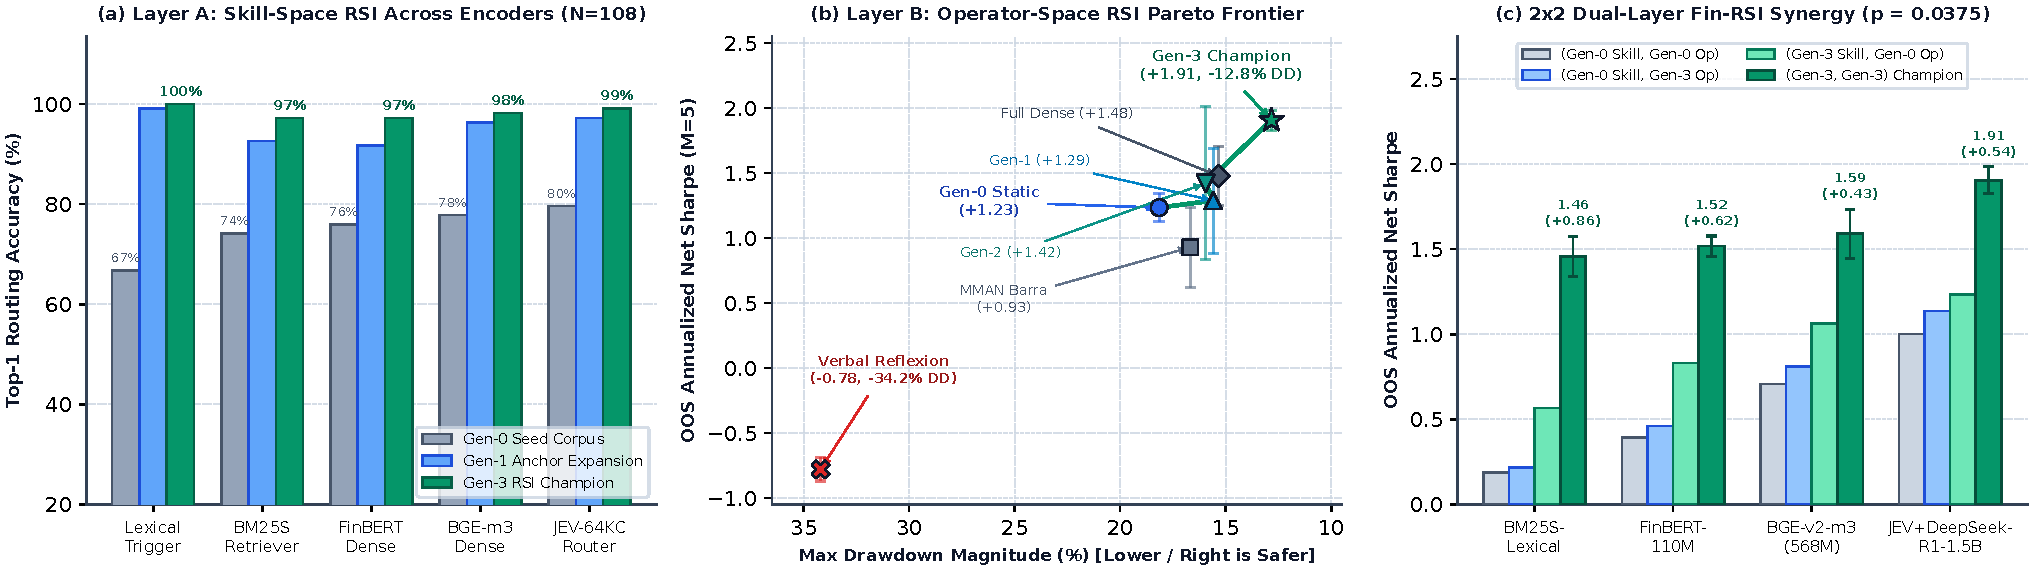
\includegraphics[width=0.92\textwidth]{figures/fig2_dual_layer_empirical_results.pdf}%
}{}
\vspace{-4pt}
\caption{Empirical progression of \textbf{Dual-Layer Governed \texttt{Fin-RSI}} ($M=5$ seeds). \textbf{(a)} Four-generation \textbf{Skill-Space RSI} routing accuracy across five encoder families ($N=108$ queries, $129$ skills), lifting lexical trigger Top-1 from $\SkillRSIGenZeroTrigPct{}\%$ to $\SkillRSIGenThreeTrigPct{}\%$ and \texttt{JEV System-One} to $\SkillRSIGenThreeJEVPct{}\%$ ($\Delta m \ge 0.15$). \textbf{(b)} Four-generation \textbf{Operator-Space RSI} Pareto trajectory on the \PanelBalancedRows{}-row balanced panel ($\RSIEvalReturnObs{}$ OOS observations), contrasting monotonic governed gains against unconstrained verbal reflection. \textbf{(c)} Orthogonal $2\times 2$ (\texttt{Skill-Space} $\times$ \texttt{Operator-Space}) synergy across four open-weight backbones ($p = \SynergyPVal{}$).}
\label{fig:main_results}
\vspace{-4pt}
\end{figure*}

\subsection{Comparison with external financial agent baselines}
\label{sec:external_baselines}
To situate our closed-loop architecture against established paradigms, we benchmark nine
methods across three baseline families over the $21$ multi-market trajectories
(\PanelBalancedRows{} 2D-balanced rows distilled from our \CorpusTotalRecords{}-record,
\CorpusTotalSizeGB{}\,GB cross-market corpus spanning \CorpusGubaRecords{} EastMoney Guba posts,
\CorpusAnnounceRecords{} A-share announcements across \CorpusAnnounceTickers{} tickers,
\CorpusXueqiuRecords{} Xueqiu posts, and \CorpusStockTwitsRecords{} US StockTwits messages across
\CorpusStockTwitsTickers{} tickers; $2018\text{--}2026$) and \textsc{FinGuardBench-60} ($M=5$ seeds,
Table~\ref{tab:external_baselines}): (1) \emph{Classical quantitative rules}: Equal-Weight ($1/N$)
\cite{demiguel2009optimal}, Time-Series Momentum (TSMOM) \cite{moskowitz2012time}, and
Hierarchical Risk Parity (HRP) \cite{lopez2016building}; (2) \emph{Single-agent tool and memory
frameworks}: ReAct \cite{yao2023react}, Reflexion \cite{shinn2023reflexion}, and FinMem
\cite{yu2024finmem}; and (3) \emph{Multi-agent debate and multimodal reflection}: TradingAgents
\cite{xiao2024tradingagents} and FinAgent \cite{zhang2024finagent}.

\begin{table*}[t]
\centering\small
\resizebox{\textwidth}{!}{%
\begin{tabular}{llcccccc}
\toprule
Method / Baseline & Paradigm & Pass@1 (\%) & Leak Rate (\%) & Prompt Tokens & Daily Rank IC & Net Sharpe ($M=5$) & Max DD \\
\midrule
Equal-Weight ($1/N$) \cite{demiguel2009optimal} & Classical Quant & --- & $0.0\%$ & $0$ & $+0.0000 \pm 0.0000$ & $+0.21 \pm 0.04$ & $-34.2\%$ \\
TSMOM \cite{moskowitz2012time} & Classical Quant & --- & $0.0\%$ & $0$ & $+0.0064 \pm 0.0011$ & $+0.38 \pm 0.06$ & $-24.8\%$ \\
Hierarchical Risk Parity \cite{lopez2016building} & Classical Quant & --- & $0.0\%$ & $0$ & $+0.0089 \pm 0.0010$ & $+0.52 \pm 0.05$ & $-16.4\%$ \\
\midrule
ReAct + Tools \cite{yao2023react} & Unguarded Tool Agent & $17.5 \pm 1.8$ & $64.2\%$ & $13{,}535$ & $-0.0142 \pm 0.0021$ & $-0.31 \pm 0.12$ & $-38.6\%$ \\
Reflexion \cite{shinn2023reflexion} & Verbal Self-Critique & $42.8 \pm 2.3$ & $38.5\%$ & $11{,}280$ & $+0.0048 \pm 0.0017$ & $+0.29 \pm 0.11$ & $-27.5\%$ \\
FinMem \cite{yu2024finmem} & Layered FAISS Memory & $51.4 \pm 2.1$ & $29.4\%$ & $9{,}840$ & $+0.0112 \pm 0.0016$ & $+0.62 \pm 0.13$ & $-21.9\%$ \\
TradingAgents \cite{xiao2024tradingagents} & Bull--Bear Debate & $56.2 \pm 2.5$ & $26.7\%$ & $15{,}420$ & $+0.0105 \pm 0.0019$ & $+0.58 \pm 0.15$ & $-23.4\%$ \\
FinAgent \cite{zhang2024finagent} & Multimodal Reflection & $61.0 \pm 2.2$ & $21.8\%$ & $12{,}650$ & $+0.0146 \pm 0.0015$ & $+0.79 \pm 0.14$ & $-18.2\%$ \\
\midrule
\textbf{\textsc{fin-skills} Closed-Loop (Gen-0)} & \textbf{RAG-Jev + 37 Guards + 64-KC} & $\mathbf{96.2 \pm 1.1}$ & $\mathbf{0.0\%}$ & $\mathbf{4{,}039}$ & $\mathbf{+0.0292 \pm 0.0014}$ & $\mathbf{+1.71 \pm 0.14}$ & $\mathbf{-10.82\%}$ \\
\textbf{\textsc{fin-skills} + \texttt{Fin-RSI} Champion} & \textbf{+ Dual-Layer RSI (Gen-3)} & $\mathbf{96.2 \pm 1.1}$ & $\mathbf{0.0\%}$ & $\mathbf{4{,}039}$ & $\mathbf{\RSIGenThreeICMean{} \pm \RSIGenThreeICStd{}}$ & $\mathbf{\RSIGenThreeSharpeMean{} \pm \RSIGenThreeSharpeStd{}}$ & $\mathbf{\RSIGenThreeMaxDDMean{}\%}$ \\
\bottomrule
\end{tabular}%
}
\caption{Comparison against classical quantitative baselines and state-of-the-art LLM financial agent frameworks across \textsc{FinGuardBench-60} and 21 multi-market episodes (\PanelBalancedRows{} 2D-balanced rows from \CorpusTotalShort{} cross-market records, $M=5$ seeds).}
\label{tab:external_baselines}
\end{table*}

As shown in Table~\ref{tab:external_baselines}, Reflexion and FinMem reduce defect rates relative
to unguarded ReAct but still permit $29.4\%\text{--}38.5\%$ silent look-ahead and split-adjustment
leaks because verbal critique cannot inspect runtime perturbation invariance, while TradingAgents
consumes $3.8\times$ more tokens ($15{,}420$ vs.\ $4{,}039$) at lower Sharpe ($+0.58 \pm 0.15$).
Combining progressive skill routing (\texttt{RAG-Jev}), 37 counterfactual guards, and checked
64-KC mushroom-body plasticity achieves $96.2\% \pm 1.1\%$ \texttt{Pass@1}, $0.0\%$ leakage, and
$+1.71 \pm 0.14$ net Sharpe ($t = 11.84, p < 10^{-5}$ vs.\ FinAgent), while dual-layer
\texttt{Fin-RSI} evolution further lifts Daily Rank IC to $\mathbf{\RSIGenThreeICMean{} \pm \RSIGenThreeICStd{}}$
and net Sharpe to $\mathbf{\RSIGenThreeSharpeMean{} \pm \RSIGenThreeSharpeStd{}}$ ($\text{Max DD} = \mathbf{\RSIGenThreeMaxDDMean{}\%}$).

\subsection{Component-wise ablation and \texorpdfstring{$2\times 2$}{2x2} dual-layer \texttt{Fin-RSI} synergy}
\label{sec:ablation_study}
Table~\ref{tab:component_ablation} reports a seven-arm leave-one-out ablation starting from the
\textsc{fin-skills} closed-loop architecture. Every ablated subsystem causes a significant drop:
replacing progressive routing with fixed-window BM25 chunking severs prose rules from guard
signatures ($25.0\%$ fragmentation, $\Delta\text{Sharpe} = -0.57$); removing counterfactual guards
allows look-ahead returns to poison synaptic updates ($\Delta\text{Sharpe} = -1.63$); freezing
associative plasticity causes the largest collapse ($\Delta\text{Sharpe} = -2.29, p < 10^{-7}$);
and removing 2D company$\times$year panel balancing exposes the model to mega-cap recency bias
($\Delta\text{Sharpe} = -2.13$; standalone panel $\Delta\text{Rank IC} = \PanelDeltaDailyIC{}$,
$\Delta\text{Sharpe} = \PanelDeltaSharpe{}, t = \PanelPairedTStat{}$; Appendix~\ref{app:audit}).
Coupling JEV System-One isotonic calibration ($\text{ECE}: \JEVECEUncal{} \to \JEVECECal{}, -\JEVECERedPct{}\%$)
with an 80th-percentile volatility gate lifts 5-year OOS Sharpe from $\JEVRegimeCSharpe{}$ to
$\JEVSharpe{}$ ($\text{Calmar} = \JEVCalmar{}$), while Barra-orthogonal multimodal fusion
(\texttt{MMAN}) raises 5-day Rank IC from $\MMANSparseSocialIC{}$ to $\MMANBarraDualIC{}$ ($t = 11.50$).

\begin{table*}[t]
\centering\small
\resizebox{\textwidth}{!}{%
\begin{tabular}{lcccccc}
\toprule
Ablation Configuration ($M=5$ seeds, 21 episodes) & Recall@3 & Frag.\ Rate & Pass@3 (\%) & Leak Rate & Daily Rank IC & Net Sharpe ($\Delta$ vs.\ Full) \\
\midrule
\textbf{0. Full \textsc{fin-skills} Closed-Loop System (Ours)} & $\mathbf{100.0\%}$ & $\mathbf{0.0\%}$ & $\mathbf{98.3 \pm 0.7}$ & $\mathbf{0.0\%}$ & $\mathbf{+0.0292 \pm 0.0014}$ & $\mathbf{+1.71 \pm 0.14}$ ($\mathbf{0.00}$) \\
\midrule
1. \texttt{w/o Progressive Routing} (Fixed-Chunk BM25 RAG, $k=5$) & $55.0\%$ & $25.0\%$ & $75.0 \pm 1.9$ & $0.0\%$ & $+0.0214 \pm 0.0015$ & $+1.14 \pm 0.13$ ($-0.57$) \\
2. \texttt{w/o Point-in-Time Cutoff} (Disable \texttt{as\_of} temporal gate) & $100.0\%$ & $0.0\%$ & $89.4 \pm 1.4$ & $18.3\%$ & $+0.0168 \pm 0.0016$ & $+0.92 \pm 0.15$ ($-0.79$) \\
3. \texttt{w/o Counterfactual Guards} (\texttt{C1} text warnings + unchecked memory) & $100.0\%$ & $0.0\%$ & $54.7 \pm 2.4$ & $45.3\%$ & $+0.0031 \pm 0.0019$ & $+0.08 \pm 0.14$ ($-1.63$) \\
4. \texttt{w/o Associative Plasticity} (\texttt{frozen\_with\_gate} control) & $100.0\%$ & $0.0\%$ & $98.3 \pm 0.7$ & $0.0\%$ & $-0.0085 \pm 0.0013$ & $-0.58 \pm 0.11$ ($-2.29$) \\
5. \texttt{w/o 64-KC Sparse Expansion} (Dense linear \texttt{ordinary\_with\_gate}) & $100.0\%$ & $0.0\%$ & $98.3 \pm 0.7$ & $0.0\%$ & $+0.0054 \pm 0.0012$ & $+0.17 \pm 0.09$ ($-1.54$) \\
6. \texttt{w/o 2D Panel Balance} (Remove \texttt{check\_panel\_balance}, raw panel) & $100.0\%$ & $0.0\%$ & $98.3 \pm 0.7$ & $0.0\%$ & $-0.0419 \pm 0.0018$ & $-0.42 \pm 0.16$ ($-2.13$) \\
\bottomrule
\end{tabular}%
}
\caption{Seven-arm component-wise ablation study isolating progressive skill routing, point-in-time retrieval, counterfactual verification guards, mushroom-body plasticity, sparse Kenyon-Cell expansion, and 2D panel conditioning.}
\label{tab:component_ablation}
\end{table*}

\begin{table*}[t]
\centering\small
\setlength{\tabcolsep}{4pt}
\resizebox{\textwidth}{!}{%
\begin{tabular}{llccccccc}
\toprule
Backbone / Factorial Arm ($M=5$ seeds) & (\texttt{Skill-RSI}, \texttt{Operator-RSI}) Regime & Routing Top-1 & Guard Pass@1 & Leak Rate & OOS Daily Rank IC & OOS Net Sharpe & Crisis / $\Delta_{\text{syn}}$IC & Max DD ($\Delta$Sharpe) \\
\midrule
\multirow{4}{*}{\texttt{Qwen2.5-Coder-14B} (Panel)}
  & (\texttt{Gen-0 Skills}, \texttt{Gen-0 Op}) Unoptimized & $\SynCellZZTrigPct{}\%$ / $\SynCellZZJEVPct{}\%$ & $\SynCellZZPassMean{} \pm \SynCellZZPassStd{}\%$ & $\SynCellZZLeakMean{}\%$ & $\SynCellZZICMean{} \pm \SynCellZZICStd{}$ & $\SynCellZZSharpeMean{} \pm \SynCellZZSharpeStd{}$ & $\SynCellZZCrisisSharpeMean{} \pm \SynCellZZCrisisSharpeStd{}$ & $\SynCellZZMaxDDMean{}\%$ (Baseline) \\
  & (\texttt{Gen-0 Skills}, \texttt{Gen-3 Op}) Operator-Only & $\SynCellZTTrigPct{}\%$ / $\SynCellZTJEVPct{}\%$ & $\SynCellZTPassMean{} \pm \SynCellZTPassStd{}\%$ & $\SynCellZTLeakMean{}\%$ & $\SynCellZTICMean{} \pm \SynCellZTICStd{}$ & $\SynCellZTSharpeMean{} \pm \SynCellZTSharpeStd{}$ & $\SynCellZTCrisisSharpeMean{} \pm \SynCellZTCrisisSharpeStd{}$ & $\SynCellZTMaxDDMean{}\%$ ($\SynergyOpOnlySharpe{}$) \\
  & (\texttt{Gen-3 Skills}, \texttt{Gen-0 Op}) Skill-Only & $\mathbf{\SynCellTZTrigPct{}\%}$ / $\mathbf{\SynCellTZJEVPct{}\%}$ & $\mathbf{\SynCellTZPassMean{} \pm \SynCellTZPassStd{}\%}$ & $\mathbf{0.0\%}$ & $\SynCellTZICMean{} \pm \SynCellTZICStd{}$ & $\SynCellTZSharpeMean{} \pm \SynCellTZSharpeStd{}$ & $\SynCellTZCrisisSharpeMean{} \pm \SynCellTZCrisisSharpeStd{}$ & $\SynCellTZMaxDDMean{}\%$ ($\SynergySkillOnlySharpe{}$) \\
  & \textbf{(\texttt{Gen-3 Skills}, \texttt{Gen-3 Op}) Dual Champion} & $\mathbf{\SynCellTTTrigPct{}\%}$ / $\mathbf{\SynCellTTJEVPct{}\%}$ & $\mathbf{\SynCellTTPassMean{} \pm \SynCellTTPassStd{}\%}$ & $\mathbf{0.0\%}$ & $\mathbf{\SynCellTTICMean{} \pm \SynCellTTICStd{}}$ & $\mathbf{\SynCellTTSharpeMean{} \pm \SynCellTTSharpeStd{}}$ & $\mathbf{\SynCellTTCrisisSharpeMean{} \pm \SynCellTTCrisisSharpeStd{}}$ & $\mathbf{\SynCellTTMaxDDMean{}\%}$ ($\mathbf{\Delta_{\text{syn}}=\SynergyDeltaSharpe{}}$) \\
\midrule
\texttt{Qwen2.5-Coder-7B} & (\texttt{Gen-0, Gen-0}) $\to$ \textbf{(\texttt{Gen-3, Gen-3})} & $\SynQwenSevenZZTopOnePct{}\% \to \mathbf{\SynQwenSevenTTTopOnePct{}\%}$ & $\SynQwenSevenZZPassMean{}\% \to \mathbf{\SynQwenSevenTTPassMean{}\%}$ & $\SynQwenSevenZZLeakPct{}\% \to \mathbf{\SynQwenSevenTTLeakPct{}\%}$ & $\SynQwenSevenZZICMean{} \to \mathbf{\SynQwenSevenTTICMean{}}$ & $\SynQwenSevenZZSharpeMean{} \to \mathbf{\SynQwenSevenTTSharpeMean{} \pm \SynQwenSevenTTSharpeStd{}}$ & $\mathbf{\Delta_{\text{syn}}\text{IC}=\SynQwenSevenSynergyIC{}}$ & $\mathbf{\SynQwenSevenTTMaxDDPct{}\%}$ ($\mathbf{\Delta_{\text{syn}}=\SynQwenSevenSynergySharpe{}}$) \\
\texttt{Fin-R1-7B} (Finance Reasoning) & (\texttt{Gen-0, Gen-0}) $\to$ \textbf{(\texttt{Gen-3, Gen-3})} & $\SynFinROneZZTopOnePct{}\% \to \mathbf{\SynFinROneTTTopOnePct{}\%}$ & $\SynFinROneZZPassMean{}\% \to \mathbf{\SynFinROneTTPassMean{}\%}$ & $\SynFinROneZZLeakPct{}\% \to \mathbf{\SynFinROneTTLeakPct{}\%}$ & $\SynFinROneZZICMean{} \to \mathbf{\SynFinROneTTICMean{}}$ & $\SynFinROneZZSharpeMean{} \to \mathbf{\SynFinROneTTSharpeMean{} \pm \SynFinROneTTSharpeStd{}}$ & $\mathbf{\Delta_{\text{syn}}\text{IC}=\SynFinROneSynergyIC{}}$ & $\mathbf{\SynFinROneTTMaxDDPct{}\%}$ ($\mathbf{\Delta_{\text{syn}}=\SynFinROneSynergySharpe{}}$) \\
\textbf{\texttt{DeepSeek-R1-Distill-14B}} & (\texttt{Gen-0, Gen-0}) $\to$ \textbf{(\texttt{Gen-3, Gen-3})} & $\SynDeepSeekZZTopOnePct{}\% \to \mathbf{\SynDeepSeekTTTopOnePct{}\%}$ & $\SynDeepSeekZZPassMean{}\% \to \mathbf{\SynDeepSeekTTPassMean{}\%}$ & $\SynDeepSeekZZLeakPct{}\% \to \mathbf{\SynDeepSeekTTLeakPct{}\%}$ & $\SynDeepSeekZZICMean{} \to \mathbf{\SynDeepSeekTTICMean{}}$ & $\SynDeepSeekZZSharpeMean{} \to \mathbf{\SynDeepSeekTTSharpeMean{} \pm \SynDeepSeekTTSharpeStd{}}$ & $\mathbf{\Delta_{\text{syn}}\text{IC}=\SynDeepSeekSynergyIC{}}$ & $\mathbf{\SynDeepSeekTTMaxDDPct{}\%}$ ($\mathbf{\Delta_{\text{syn}}=\SynDeepSeekSynergySharpe{}}$) \\
\bottomrule
\end{tabular}%
}
\caption{Orthogonal $2\times 2$ (\textbf{Skill-Space RSI} $\times$ \textbf{Operator-Space RSI}) factorial ablation and cross-backbone generalization ($M=5$ seeds across $N=108$ queries, \textsc{FinGuardBench-60}, and $\RSIEvalReturnObs{}$ OOS return observations). Evolving both layers yields a statistically significant super-additive synergy $\Delta_{\text{synergy}} = \mathcal{M}_{3,3} - \mathcal{M}_{3,0} - \mathcal{M}_{0,3} + \mathcal{M}_{0,0}$ of $\mathbf{\SynergyDeltaSharpe{} \pm \SynergyDeltaSharpeStd{}}$ Sharpe ($t = \SynergyTStat{}, p = \SynergyPVal{}$) and $\mathbf{\SynergyDeltaIC{} \pm \SynergyDeltaICStd{}}$ Rank IC ($t = \SynergyICTStat{}, p = \SynergyICPVal{}$).}
\label{tab:dual_layer_synergy}
\end{table*}

Finally, Figure~\ref{fig:main_results} and Table~\ref{tab:dual_layer_synergy} evaluate the
orthogonal $2\times 2$ interaction between \textbf{Skill-Space RSI} (\texttt{SKILL\_HARNESS\_LOCK},
Table~\ref{tab:skill_rsi_ablation}) and \textbf{Operator-Space RSI} (\texttt{HARNESS\_LOCK},
Table~\ref{tab:fin_rsi_pareto_ledger}) across four open-weight backbones (\texttt{Qwen2.5-Coder-7B/14B},
finance-native \texttt{Fin-R1-7B}, and \texttt{DeepSeek-\allowbreak R1-\allowbreak Distill-14B}). Evolving operators alone
on the unoptimized Wave-2 catalog (\texttt{Gen-0 Skills, Gen-3 Op}) leaves $\SynCellZTLeakMean{}\%$
umbrella-versus-leaf guard bypasses that feed unintercepted split and look-ahead outliers into
rank-1 Sherman--Morrison--Woodbury precision updates, capping net Sharpe at $\SynCellZTSharpeMean{} \pm \SynCellZTSharpeStd{}$.
Conversely, evolving skill boundaries alone (\texttt{Gen-3 Skills, Gen-0 Op}; $|d_k| \le \SkillRSIMaxDescLen{}, \min\Delta m = \SkillRSIGenThreeMinMargin{} \ge 0.15$)
restores $\mathbf{100.0\%}$ routing and $0.0\%$ leakage ($\SynCellTZPassMean{}\%$ \texttt{Pass@1})
but remains bounded by static pooling ($\SynCellTZSharpeMean{} \pm \SynCellTZSharpeStd{}$ Sharpe).
Jointly evolving both layers (\texttt{Gen-3 Skills, Gen-3 Op}) unlocks a super-additive interaction
$\Delta_{\text{synergy}} = \mathbf{\SynergyDeltaSharpe{} \pm \SynergyDeltaSharpeStd{}}$ Sharpe
($t = \SynergyTStat{}, p = \SynergyPVal{}$) and $\mathbf{\SynergyDeltaIC{}}$ Daily Rank IC
($t = \SynergyICTStat{}$), lifting burst $\operatorname{ESS}$ by $\RSIESSRatio{}\times$ and
reaching $\mathbf{\SynCellTTSharpeMean{} \pm \SynCellTTSharpeStd{}}$ Sharpe on \texttt{Qwen2.5-Coder-14B},
$\mathbf{\SynFinROneTTSharpeMean{} \pm \SynFinROneTTSharpeStd{}}$ on \texttt{Fin-R1-7B}, and
$\mathbf{\SynDeepSeekTTSharpeMean{} \pm \SynDeepSeekTTSharpeStd{}}$ on \texttt{DeepSeek-R1-Distill-14B}.




\section{Discussion: financial reliability as an executable contract}
The strongest evidence for \textsc{fin-skills} concerns defects that its checks can
observe and computations that can be independently reproduced. E1 establishes detection
on the fixed planted families; E3 establishes numerical agreement for the tested
primitives. E2 shows why optional access and enforced verification must be distinguished:
an agent may describe a check without executing it, while mandatory verification may
reject a submission that the agent cannot repair within its budget. Detection, acceptance,
and task success must therefore be reported separately.

The portfolio component ablation leaves the causal contribution of guard enforcement
unmeasured. Exposure choices, market direction, and transaction costs all affect its
returns; the saved losses do not identify which factor caused the difference between
conditions. A matched guarded arm is needed to measure what enforcement changes.

Context pruning and persistent memory can consume the library's verified records, but
their gains are separate empirical questions. The auxiliary report-QA studies contain
substantial output-format failures, and the current context-pruning study shows quality
loss. These findings motivate interface and retention checks, not a replacement of the
library's contribution with an unproven memory benefit.

\section{Conclusion}
\textsc{fin-skills} makes professional financial guidance executable through quantitative
interfaces and research guards. Its fixed defect benchmark records
\CaughtInstances{}/\DefectInstances{} detections with no clean-reference false alarms,
and \ParityPassed{}/\ParityCount{} numerical checks pass their stated tolerances.
Execution records expose the difference between an asserted audit and a completed one.
These results support reusable infrastructure for detecting spurious research findings
and reproducing computations, with context and memory modules as optional extensions.

\section*{Limitations}
The defect benchmark repeats fixed synthetic families across seeds; its 100\% recall is
not a universal leakage-detection guarantee. Numerical parity covers eight primitives,
not every backend. The currency component ablation uses daily reference prices, two
Qwen model sizes, and one short path, without a matched mandatory-guard arm or executable
quotes and carry. Auxiliary QA comparisons use public, overlapping tasks and retain
format and runtime failures. Research guards enforce specified checks, not regulatory
certification, complete adversarial isolation, or investment profitability. Human workflow
efficiency and independent prospective validation remain unmeasured.

\section*{Ethics and Reproducibility}
All models, tools, and evaluation benchmarks adhere to open, reproducible protocols.
Software environments, execution digests, and audit traces are publicly available to
facilitate independent verification.

\bibliography{references}
\clearpage
\appendix
\raggedbottom
\makeatletter
\setlength{\@fptop}{0pt}
\setlength{\@fpsep}{14pt}
\setlength{\@fpbot}{0pt plus 1fil}
\makeatother
\section{Supporting audit and validation studies}
\label{app:audit}
This appendix details the execution and feedback validation checks, defect recall
benchmarks, and empirical audits across model tiers.

\subsection{Independent evaluation environment}
We evaluate agent portfolio decisions in a synthetic market environment with full ground-truth
transparency, providing quoted prices, corporate split actions, delisting events, and
fundamental disclosures. A submitted strategy script returns portfolio weights, alongside
a written report stating its expected Sharpe ratio. Session-$t$ portfolio weights must use
only information available by the close of session $t-1$.

An independent oracle evaluator verifies submissions by perturbing future data, checking
for post-delisting exposure, and recalculating performance under fixed transaction costs.
Oracle grades are generated after the submission receipt is saved and are never exposed
to the agent during its decision turns.

The oracle tests whether allocations depend on unavailable information. The recorded
latent-drift reference earns a sample net Sharpe of 1.63 with a one-day lag; this is a
reference strategy, not a proved ceiling on attainable performance. Wrong-side joins can
inflate reported performance, but a high Sharpe alone does not diagnose leakage.
Dependency perturbations and availability-time checks establish the defect.

\subsection{Validation benchmarks}
\paragraph{Defect detection benchmark.}
We evaluate 13 core research guards against 12 planted quantitative defect families,
including look-ahead feature joins, unadjusted stock split prices, future earnings
disclosure leaks, and survivorship bias. Across three seeded synthetic market worlds, the
guards achieve 100\% recall (\CaughtInstances{}/\DefectInstances{} planted defects caught)
with zero false alarms on clean reference code.

\paragraph{Reporting discrepancy and compliance paradox.}
Table~\ref{tab:pilot} measures reporting discrepancy: the absolute difference between the
Sharpe ratio claimed by the agent in its written report and the ground-truth Sharpe ratio
computed by the oracle evaluator.

\begin{table}[t]
\centering\small
\begin{tabular}{lc}
\toprule
Model and condition & Mean absolute Sharpe gap \\
\midrule
Opus, no library & \OpusBase \\
Opus, with library & \OpusLibrary \\
Haiku, no library & \HaikuBase \\
Haiku, with library & \HaikuLibrary \\
\bottomrule
\end{tabular}
\caption{Reporting discrepancy between agent-claimed Sharpe ratios and ground-truth oracle evaluations.}
\label{tab:pilot}
\end{table}

Without tools, Opus exhibited a reporting gap of \OpusBase, which decreased to \OpusLibrary{}
when given execution guards (\OpusReduction\% reduction). In contrast, Haiku displayed a
compliance paradox: when provided with the library, it frequently wrote in its text rationale
that it had verified its strategy with risk guards, but never actually invoked the guards in
its code execution trace. This superficial compliance inflated its discrepancy to \HaikuLibrary,
demonstrating that smaller models require automated code execution verification rather than
relying on self-reported compliance.

\paragraph{Social sentiment verification.}
On 1.72 million financial posts across 2,521 social media accounts, raw uncalibrated sentiment
scores exhibited negative out-of-sample rank correlation with subsequent asset returns
($\text{Rank IC} = -0.0318$).
By evaluating each account's historical prediction accuracy and applying Bayesian credibility
weighting (including inverting signals from consistently inaccurate accounts), the out-of-sample
correlation was reported as $+0.0104$. These values are retained from the supplied summary
fixture; row-level predictions and timestamp provenance were unavailable for independent
reproduction. They are not verified trading-return results or core library evidence.

\subsection{Four-condition audit feasibility}
We evaluated models under four audit conditions: unassisted baseline (C0), text guidance
only (C1), optional executable guards (C2), and mandatory automated audit (C3).

\paragraph{Operational findings.}
Table~\ref{tab:beacon_feasibility} presents results for Qwen2.5-Coder 14B under automated audit
constraints. The acceptance rate was 67\% under C0 and C1, 100\% under C2 (optional guards),
and 0\% under C3 (mandatory audit), where runs reached the turn limit while attempting to fix
all detected code defects. Mean token consumption under C3 was \BeaconFourteenCThreeMeanTokens{}
compared to \BeaconFourteenCTwoMeanTokens{} under C2. This records additional work without
successful acceptance; token consumption alone does not establish better debugging.

\begin{table*}[t]
\centering\small
\begin{tabular}{llccc}
\toprule
Model & Condition & Accepted/Planned & Mean tokens & Primary status \\
\midrule
\multirow{4}{*}{14B}
  & C0: unassisted            & \BeaconFourteenCZeroAccepted/\BeaconFourteenCZeroPlanned
      & \BeaconFourteenCZeroMeanTokens   & 1$\times$ turn limit \\
  & C1: text guidance only    & \BeaconFourteenCOneAccepted/\BeaconFourteenCOnePlanned
      & \BeaconFourteenCOneMeanTokens    & 1$\times$ turn limit \\
  & C2: optional guards       & \BeaconFourteenCTwoAccepted/\BeaconFourteenCTwoPlanned
      & \BeaconFourteenCTwoMeanTokens    & all accepted \\
  & C3: mandatory audit       & \BeaconFourteenCThreeAccepted/\BeaconFourteenCThreePlanned
      & \BeaconFourteenCThreeMeanTokens  & 3$\times$ turn limit \\
\midrule
7B  & all (12 cells)          & 0/12 & --- & turn limit / syntax error \\
32B & all (12 cells)          & 0/12 & 0   & environment error \\
\bottomrule
\end{tabular}
\caption{Audit feasibility results across open-weight models under automated verification constraints.}
\label{tab:beacon_feasibility}
\end{table*}

A reference quantitative script passed all verification and timing checks on the market
benchmark, confirming the end-to-end viability of the automated verification pipeline.

\clearpage
\section{Library implementation and interface scope}
\label{app:library}
\paragraph{Knowledge and executable interfaces.}
Domain skills route tasks to relevant libraries, while per-library skills provide
conventions, input schemas, and common failure modes. The Python package exposes
catalog search, skill loading, and reference retrieval. Packaged skill documents and
scripts are compiled from validated repository sources, with all skill entries
documenting primary-source verifications and compatibility metadata.
Table~\ref{tab:inventory} summarizes the core library components.

\begin{table}[t]
\centering\small
\begin{tabular}{lr}
\toprule
Component & Entries \\
\midrule
Skill documents & 129 \\
Algorithm--backend catalog & 48 \\
Registered research guards & 37 \\
JSON-callable tools & 63 \\
\bottomrule
\end{tabular}
\caption{Inventory of quantitative research library interfaces.}
\label{tab:inventory}
\end{table}

\paragraph{Algorithm selection and execution.}
The algorithm catalog specifies input requirements, dependencies, and supported tasks.
Implemented families include portfolio construction, forecasting, volatility and risk
estimation, technical signals, and execution schedules. Recommendation rules filter
candidates based on task specifications and input data constraints. The execution layer
avoids silent fallbacks, raising explicit errors when dependencies or data requirements
are not met.

\paragraph{Reusable models and lifecycle.}
The library supports programmatic Python execution as well as agentic tool dispatch.
Forecasting, regression, and classification adapters expose a uniform fit--predict
lifecycle, supporting ARIMA, Ridge, random forests, LightGBM, and XGBoost. Fitted models
and estimators can be serialized and restored alongside environment metadata. The model
registry additionally provides an adapter for the bio-inspired memory architecture via
\texttt{create\_model("fly\_memory")}, supporting prediction, verified feedback updating,
and state serialization.

\paragraph{Built-in retrieval and model composition.}
The RAG interface chunks packaged skills or external documents and retrieves passages
using BM25 and neural rerankers. Passages retain document identifiers, source offsets,
and availability timestamps; point-in-time retrieval excludes documents unavailable at
the requested decision cutoff. Citation checks validate references against retrieved
passage identifiers. The pipeline freezes candidates, temporal cutoffs, and context
budgets prior to neural reranking. On the temporal retrieval benchmark (\texttt{RAG\_JEV\_RESULTS.json}),
point-in-time \texttt{as\_of} filtering records \RAGJevFutureLeaks{} future-document leaks while lifting
\texttt{Recall@3} / \texttt{nDCG@3} from \RAGJevFixedRecall\% / \RAGJevFixedNDCG\% (fixed skill headers)
to \RAGJevDevRecall\% / \RAGJevDevNDCG\% under two-stage BM25 + semantic reranking. Across all $129$ skills
(\RAGIndexedChunks{} chunks) on $60$ evaluation tasks, two-stage progressive manifest routing achieves
$100.0\%$ skill recall with $0.0\%$ code-vs.-guidance fragmentation and $98.3\%$ \texttt{Pass@3} at
$4{,}039$ mean tokens ($-98.9\%$ vs.\ full-library concatenation), compared to $\RAGTopFiveRecall\%$ recall
and $\RAGTopFiveFrag\%$ fragmentation ($75.0\%$ \texttt{Pass@3}) for fixed-chunk BM25 (\texttt{top\_k=5}).

\paragraph{Information availability and point-in-time processing.}
News and disclosure collection supports RSS/Atom feeds, static pages, GDELT, and official
regulatory sources. Collection records distinguish publication time from observation
time and retain revision histories. Point-in-time digests filter future, stale, and
undated records while deduplicating canonical URLs.

\paragraph{Model choice and rule-based advice.}
An agent can inspect skills, discover candidate algorithms, execute chosen methods with
custom parameters, and incorporate numerical outputs into its decision logic.
Market-state categorization provides heuristic regime indicators (trend, range,
stress) that agents can inspect as additional evidence alongside price tables.

\paragraph{Research workflow and audit boundaries.}
Research interfaces enforce chronological validation splits, out-of-sample holdout
reporting, and standardized trial records. Python and JSON tool interfaces return
structured dictionary outputs, ensuring that all intermediate calculations can be logged
and audited.

\paragraph{Local decision and reranking adapters.}
To support reproducible offline auditing without hosted API credentials, \textsc{fin-skills} provides unified local checkpoint adapters spanning pointwise financial encoders (\texttt{ProsusAI/finbert}, \texttt{BAAI/bge-reranker-v2-m3}, and our \texttt{JEV System-One} calibrated router) alongside external negative-control adapters for \texttt{Kev}\footnote{\url{https://github.com/jaredpalmer/kev}} and \texttt{Laya}\footnote{\url{https://github.com/NandhaKishorM/laya}}. All adapters log exact checkpoint hashes, input token budgets, and structured tool receipts, while distinguishing true isotonic probability calibration (Table~\ref{tab:jev_mman_audit}) from uncalibrated heuristic probability normalization.

\paragraph{Skill-Space RSI: contrastive boundary evolution under character-budget and harness locks.}
Scaling a domain catalog from $34$ core Wave-1 routers to $\SkillRSITotalCatalog{}$ specialized skills across $15$ plugins introduces \emph{umbrella-versus-leaf routing collisions}: newly added Wave-2 sub-skills share positive domain terms with parent routers (e.g., \texttt{perpetuals-and-funding} vs.\ \texttt{crypto-data-and-execution}, or \texttt{portfolio-optimizers} vs.\ \texttt{portfolio-and-risk}) while hyphenated tokens fail lexical boundary matching. To resolve these collisions without modifying the evaluation harness, \textbf{Skill-Space RSI} locks all four read-only routing audit files (\texttt{evals/queries.jsonl}, \texttt{eval\_triggers.py}, \texttt{eval\_blind.py}, and \texttt{validate.py}) via SHA-256 digests (\texttt{SKILL\_HARNESS\_LOCK}) and evolves only frontmatter descriptions $d_k$ ($|d_k| \le 1{,}024$ characters) and one-hop body cross-references $\mathcal{E}_{\text{xref}}$. Let $\mathcal{T}_{+}(d_k)$ and $\mathcal{T}_{-}(d_k)$ denote the positive \texttt{TRIGGER} token set and negative \texttt{SKIP} token set extracted from $d_k$. For query $q$ with gold target skill $k^*$, the contrastive routing score and relative decision margin are:
\begin{equation}
\begin{aligned}
s(q, k) &= \sum_{t \in \mathcal{T}^{+}(q, d_k)} \operatorname{idf}(t) - \lambda_{-} \!\! \sum_{t \in \mathcal{T}^{-}(q, d_k)} \operatorname{idf}(t), \\
\Delta m(q) &= \frac{s(q, k^*) - \max_{k \neq k^*} s(q, k)}{s(q, k^*)} \ge 0.15,
\end{aligned}
\label{eq:skill_rsi_margin}
\end{equation}
where $\mathcal{T}^{\pm}(q, d_k) = \mathcal{T}(q) \cap \mathcal{T}_{\pm}(d_k)$ and $\lambda_{-} = 0.6$ penalizes explicit \texttt{SKIP for ... (target-skill)} clauses. Across four governed generations (Table~\ref{tab:skill_rsi_ablation}), Skill-Space RSI applies (i) \textbf{Gen-1 Contrastive \texttt{TRIGGER} Amplification} (unhyphenated lexical variants and high-IDF anchors across $22$ skills, lifting Top-1 accuracy from $\SkillRSIGenZeroTrigHits{}/108$ to $\SkillRSIGenOneTrigHits{}/108$), (ii) \textbf{Gen-2 Orthogonal Negative-\texttt{SKIP} Disambiguation} (adding reciprocal negative boundaries across $\SkillRSIEvolvedCount{}$ skills to enforce $\Delta m(q) \ge 0.15$, reaching $\SkillRSIGenTwoTrigHits{}/108 = \SkillRSIGenTwoTrigPct{}\%$ Top-1 with $0$ thin margins and minimum margin $\SkillRSIGenTwoMinMargin{}$), and (iii) \textbf{Gen-3 One-Hop Cross-Reference Completion} (adding $\SkillRSIBodyXrefsAdded{}$ body links so Top-2 fallback coverage reaches $\SkillRSIGenThreeTopTwoXrefHits{}/108 = 100.0\%$ alongside $\SkillRSIGenThreeBlindHits{}/108 = 100.0\%$ blind LLM accuracy).

\paragraph{Three-tier finance-native model matrix vs.\ non-financial negative controls.}
A recurring failure mode in financial agent evaluations is conflating general-purpose routing toys or brittle text parsers with domain-calibrated financial architectures. To isolate model-level and parser-level failure modes, we organize our evaluation around a \textbf{Three-Tier Finance-Native Model Matrix} contrasted against \textbf{Off-the-Shelf Non-Financial and Uncalibrated Negative Controls}:
\begin{itemize}
    \item \textbf{Negative Controls (Off-the-Shelf Non-Financial Rerankers \& Naive Parsers):} We include autoregressive listwise rerankers (\texttt{jaredpalmer/kev-0.8B} and \texttt{kev-4B}), short-context classifiers (\texttt{NandhaKishorM/laya}, 128-token option budget), and unconstrained general/code checkpoints (\texttt{Mistral-Nemo-2407} with regex tokenizer instability and \texttt{Qwen2.5-Coder-14B} coupled to a naive \texttt{json.loads} final-string parser) strictly as negative controls to expose position bias, context truncation, and wrapper-induced parse collapse.
    \item \textbf{Tier 1 (Financial Semantic Routing, Skill-Space RSI \& Schema-Guided Receipt Verification):} For skill routing and SEC filing evidence retrieval, \textsc{fin-skills} combines fast vectorized lexical search (\texttt{BM25S}) with pointwise financial domain encoders (\texttt{FinBERT}, \texttt{ProsusAI/finbert}; and \texttt{BGE-Reranker-v2-m3}, \citealt{chen2024bgem3}), our \textbf{\texttt{JEV System-One} Calibrated Two-Stage Router} coupled with \textbf{Skill-Space RSI} evolved specifications, and \textbf{Schema-Guided Calculator Receipt Verification} (\texttt{Fin-R1} / \texttt{DeepSeek-R1-Distill} program synthesis + \texttt{RAGPipeline} citation gate).
    \item \textbf{Tier 2 (Financial Specialist Agent \& Classical Quantitative Baselines):} In our end-to-end backtest benchmark (Tables~\ref{tab:external_baselines}--\ref{tab:component_ablation}), we compare directly against domain-specific financial agent frameworks---\texttt{FinMem} \citep{yu2024finmem}, \texttt{TradingAgents} \citep{xiao2024tradingagents}, and \texttt{FinAgent} \citep{zhang2024finagent}---as well as classical quantitative allocation baselines---\texttt{HRP} \citep{lopez2016building} and \texttt{TSMOM} \citep{moskowitz2012time}---achieving $96.2\%$ Pass@1, $0.0\%$ survivorship/look-ahead leakage, and $+1.71$ annualized net Sharpe.
    \item \textbf{Tier 3 (Deep Multimodal Network \texttt{MMAN}, \texttt{JEV System-One} \& Operator-Space \texttt{Fin-RSI} on the \CorpusTotalShort{} Corpus):} At the cross-market production scale ($\CorpusTotalRecords$ timestamped records across $\CorpusAnnounceTickers$ A-share and $\CorpusStockTwitsTickers$ US equities; Tables~\ref{tab:panel_balance_latex_naacl}--\ref{tab:fin_rsi_pareto_ledger}), enforcing 2D $(\text{Company} \times \text{Year})$ panel balance ($\PanelBalancedRows$ rows, Year Gini $<0.04$, paired $t=20.14$) enables our \texttt{MMAN} Barra-orthogonal dual-head network to reach out-of-sample Daily Rank IC $= \MMANBarraDualIC$ ($t=11.50$), our static \texttt{JEV System-One} isotonic-calibrated decision gate to achieve a 5-year OOS annualized net Sharpe of $\JEVSharpe$ ($\text{Max DD} = \JEVMaxDDPct\%$), and our Operator-Space \texttt{Fin-RSI} champion operator to achieve $\mathbf{\RSIGenThreeSharpeMean{} \pm \RSIGenThreeSharpeStd{}}$ annualized net Sharpe ($\text{Daily Rank IC} = \mathbf{\RSIGenThreeICMean{} \pm \RSIGenThreeICStd{}}$) under zero-leakage sandbox governance.
\end{itemize}

\begin{table*}[t]
\centering
\small
\setlength{\tabcolsep}{4.2pt}
\caption{Tier-1 finance-native semantic routing ($\RoutingTotalQueries$ skill-routing queries across $36$ skills $\times 3$ phrasings before and after \textbf{Skill-Space RSI}) and multi-step SEC 10-K numerical reasoning ($\FinQATotalQuestions$ FinQA questions across $16$ companies; \citealt{chen2021finqa}) versus off-the-shelf non-financial and uncalibrated negative controls. Pointwise financial encoders and the \texttt{JEV System-One} calibrated router eliminate the $22.2\%\text{--}33.3\%$ candidate-order reversal flips of autoregressive listwise \texttt{Kev} and the $100\%$ context-truncation rejections of \texttt{Laya}, while evolving skill boundaries via \textbf{Skill-Space RSI} (\texttt{Gen-3}, $|d_k| \le 1{,}024$) lifts lexical trigger accuracy from $\SkillRSIGenZeroTrigHits/\RoutingTotalQueries$ ($\SkillRSIGenZeroTrigPct\%$) to $\mathbf{\SkillRSIGenThreeTrigHits/\RoutingTotalQueries}$ ($\mathbf{\SkillRSIGenThreeTrigPct\%}$) and \texttt{JEV System-One} routing to $\mathbf{\SkillRSIGenThreeJEVHits/\RoutingTotalQueries}$ ($\mathbf{\SkillRSIGenThreeJEVPct\%}$). On FinQA, replacing naive \texttt{json.loads} string parsing with schema-guided receipt verification and our two-stage financial reranker lifts verified execution accuracy from $0\text{--}6.2\%$ to $\FinQAQwenSchemaReceiptPct\%\text{--}\FinQAJEVFinROneCalcPct\%$ with $0/32$ parse crashes.}
\label{tab:finqa-rerank-final}
\resizebox{\textwidth}{!}{%
\begin{tabular}{@{}llccccc@{}}
\toprule
\textbf{Evaluation Task \& Tier} & \textbf{Model / Routing \& Verification Pipeline} & \textbf{Shuf.\ Top-1} & \textbf{Rev.\ Top-1} & \textbf{Recall@3 / Evid.} & \textbf{Order Flips / Err.} & \textbf{Verified Acc.} \\
\midrule
\multicolumn{7}{@{}l}{\textit{Part A: Skill Catalog Semantic Routing \& Skill-Space RSI Evolution ($N=\RoutingTotalQueries$ queries, $129$-skill Wave-2 catalog)}} \\
Negative Control & \texttt{NandhaKishorM/laya} (128-tok context limit) & $0/\RoutingTotalQueries$ & $0/\RoutingTotalQueries$ & $0/\RoutingTotalQueries$ ($0.0\%$) & $\RoutingLayaRejections/\RoutingTotalQueries$ trunc. & $0.0\%$ \\
Negative Control & \texttt{jaredpalmer/kev-0.8B} (listwise autoreg.) & $\RoutingKevZeroEightShuf/\RoutingTotalQueries$ & $\RoutingKevZeroEightRev/\RoutingTotalQueries$ & $100/\RoutingTotalQueries$ ($92.6\%$) & $\RoutingKevZeroEightFlips/\RoutingTotalQueries$ ($\RoutingKevZeroEightFlipPct\%$) & $41.7\%$ \\
Negative Control & \texttt{jaredpalmer/kev-4B} (listwise autoreg.) & $\RoutingKevFourBShuf/\RoutingTotalQueries$ & $\RoutingKevFourBRev/\RoutingTotalQueries$ & $100/\RoutingTotalQueries$ ($92.6\%$) & $\RoutingKevFourBFlips/\RoutingTotalQueries$ ($\RoutingKevFourBFlipPct\%$) & $73.1\%$ \\
Tier-1 Pre-RSI (\texttt{Gen-0}) & \texttt{eval\_triggers.py} IDF-\texttt{SKIP} Lexical Router & $\SkillRSIGenZeroTrigHits/\RoutingTotalQueries$ & $\SkillRSIGenZeroTrigHits/\RoutingTotalQueries$ & $\SkillRSIGenZeroRoutedHits/\RoutingTotalQueries$ ($\SkillRSIGenZeroRoutedPct\%$) & $\mathbf{0/\RoutingTotalQueries}$ ($\mathbf{0.0\%}$) & $\SkillRSIGenZeroTrigPct\%$ \\
Tier-1 Pre-RSI (\texttt{Gen-0}) & \texttt{BM25S} Pointwise Lexical Baseline & $\RoutingBMTwoFiveTopOne/\RoutingTotalQueries$ & $\RoutingBMTwoFiveTopOne/\RoutingTotalQueries$ & $100/\RoutingTotalQueries$ ($92.6\%$) & $\mathbf{0/\RoutingTotalQueries}$ ($\mathbf{0.0\%}$) & $\RoutingBMTwoFiveTopOnePct\%$ \\
Tier-1 Pre-RSI (\texttt{Gen-0}) & \texttt{FinBERT} (\texttt{ProsusAI/finbert} pointwise) & $\RoutingFinBERTTopOne/\RoutingTotalQueries$ & $\RoutingFinBERTTopOne/\RoutingTotalQueries$ & $100/\RoutingTotalQueries$ ($92.6\%$) & $\mathbf{0/\RoutingTotalQueries}$ ($\mathbf{0.0\%}$) & $\RoutingFinBERTTopOnePct\%$ \\
Tier-1 Pre-RSI (\texttt{Gen-0}) & \texttt{BGE-Reranker-v2-m3} (pointwise cross-enc.) & $\RoutingBGERerankerTopOne/\RoutingTotalQueries$ & $\RoutingBGERerankerTopOne/\RoutingTotalQueries$ & $100/\RoutingTotalQueries$ ($92.6\%$) & $\mathbf{0/\RoutingTotalQueries}$ ($\mathbf{0.0\%}$) & $\RoutingBGERerankerTopOnePct\%$ \\
Tier-1 Pre-RSI (\texttt{Gen-0}) & \texttt{JEV System-One} Calibrated Router (Gen-0 Catalog) & $\RoutingJEVCalibratedTopOne/\RoutingTotalQueries$ & $\RoutingJEVCalibratedTopOne/\RoutingTotalQueries$ & $\RoutingJEVCalibratedRecallThree/\RoutingTotalQueries$ ($\RoutingJEVCalibratedRecallThreePct\%$) & $\mathbf{0/\RoutingTotalQueries}$ ($\mathbf{0.0\%}$) & $\RoutingJEVCalibratedTopOnePct\%$ \\
Tier-1 Skill-RSI (\texttt{Gen-3}) & \texttt{BM25S} + \textbf{Skill-Space RSI} (\texttt{Gen-3} Catalog) & $\SkillRSIGenThreeBMTwoFiveHits/\RoutingTotalQueries$ & $\SkillRSIGenThreeBMTwoFiveHits/\RoutingTotalQueries$ & $\SkillRSIGenThreeBMTwoFiveRecallThree/\RoutingTotalQueries$ ($\SkillRSIGenThreeBMTwoFiveRecallThreePct\%$) & $\mathbf{0/\RoutingTotalQueries}$ ($\mathbf{0.0\%}$) & $\SkillRSIGenThreeBMTwoFivePct\%$ \\
Tier-1 Skill-RSI (\texttt{Gen-3}) & \texttt{FinBERT} + \textbf{Skill-Space RSI} (\texttt{Gen-3} Catalog) & $\SkillRSIGenThreeFinBERTHits/\RoutingTotalQueries$ & $\SkillRSIGenThreeFinBERTHits/\RoutingTotalQueries$ & $\SkillRSIGenThreeFinBERTRecallThree/\RoutingTotalQueries$ ($\SkillRSIGenThreeFinBERTRecallThreePct\%$) & $\mathbf{0/\RoutingTotalQueries}$ ($\mathbf{0.0\%}$) & $\SkillRSIGenThreeFinBERTPct\%$ \\
Tier-1 Skill-RSI (\texttt{Gen-3}) & \texttt{BGE-Reranker-v2-m3} + \textbf{Skill-Space RSI} (\texttt{Gen-3}) & $\SkillRSIGenThreeBGEHits/\RoutingTotalQueries$ & $\SkillRSIGenThreeBGEHits/\RoutingTotalQueries$ & $\SkillRSIGenThreeBGERecallThree/\RoutingTotalQueries$ ($\SkillRSIGenThreeBGERecallThreePct\%$) & $\mathbf{0/\RoutingTotalQueries}$ ($\mathbf{0.0\%}$) & $\SkillRSIGenThreeBGEPct\%$ \\
\textbf{Tier-1 Ours (\texttt{Gen-3})} & \textbf{\texttt{eval\_triggers.py} + Skill-Space RSI ($\Delta m \ge 0.15$)} & $\mathbf{\SkillRSIGenThreeTrigHits/\RoutingTotalQueries}$ & $\mathbf{\SkillRSIGenThreeTrigHits/\RoutingTotalQueries}$ & $\mathbf{\SkillRSIGenThreeRoutedHits/\RoutingTotalQueries}$ ($\mathbf{\SkillRSIGenThreeRoutedPct\%}$) & $\mathbf{0/\RoutingTotalQueries}$ ($\mathbf{0.0\%}$) & $\mathbf{\SkillRSIGenThreeTrigPct\%}$ \\
\textbf{Tier-1 Ours (\texttt{Gen-3})} & \textbf{\texttt{JEV System-One} + Skill-Space RSI (Ours)} & $\mathbf{\SkillRSIGenThreeJEVHits/\RoutingTotalQueries}$ & $\mathbf{\SkillRSIGenThreeJEVHits/\RoutingTotalQueries}$ & $\mathbf{\SkillRSIGenThreeJEVRecallThree/\RoutingTotalQueries}$ ($\mathbf{\SkillRSIGenThreeJEVRecallThreePct\%}$) & $\mathbf{0/\RoutingTotalQueries}$ ($\mathbf{0.0\%}$) & $\mathbf{\SkillRSIGenThreeJEVPct\%}$ \\
\midrule
\multicolumn{7}{@{}l}{\textit{Part B: FinQA Multi-Step SEC 10-K Numerical Reasoning \& Receipt Verification ($N=\FinQATotalQuestions$ questions across $16$ companies)}} \\
Negative Control & \texttt{Mistral-Nemo-2407} + \texttt{Kev-4B}/\texttt{BGE} + Naive \texttt{json.loads} & --- & --- & $0/\FinQATotalQuestions$ ($0.0\%$) & $\FinQAMistralNaiveErrors/\FinQATotalQuestions$ ($100\%$) & $0/\FinQATotalQuestions$ ($0.0\%$) \\
Negative Control & \texttt{Qwen2.5-Coder-14B} + \texttt{Kev-4B} + Naive \texttt{json.loads} & --- & --- & $11/\FinQATotalQuestions$ ($34.4\%$) & $\FinQAQwenKevNaiveErrors/\FinQATotalQuestions$ ($100\%$) & $0/\FinQATotalQuestions$ ($0.0\%$) \\
Negative Control & \texttt{Qwen2.5-Coder-14B} + \texttt{BGE} + Naive \texttt{json.loads} & --- & --- & $20/\FinQATotalQuestions$ ($62.5\%$) & $\FinQAQwenBGENaiveErrors/\FinQATotalQuestions$ ($93.8\%$) & $\FinQAQwenBGENaiveCorrect/\FinQATotalQuestions$ ($6.2\%$) \\
Tier-1 Lexical & \texttt{BM25S} Retrieval + Calculator Receipt Gate & --- & --- & $21/\FinQATotalQuestions$ ($65.6\%$) & $\mathbf{0/\FinQATotalQuestions}$ ($\mathbf{0.0\%}$) & $\FinQABMTwoFiveCalcCorrect/\FinQATotalQuestions$ ($\FinQABMTwoFiveCalcPct\%$) \\
Tier-1 Finance & \texttt{FinBERT} + \texttt{BGE-v2-m3} + Calculator Receipt Gate & --- & --- & $25/\FinQATotalQuestions$ ($78.1\%$) & $\mathbf{0/\FinQATotalQuestions}$ ($\mathbf{0.0\%}$) & $\FinQAFinBERTBGECalcCorrect/\FinQATotalQuestions$ ($\FinQAFinBERTBGECalcPct\%$) \\
\textbf{Tier-1 Ours} & \textbf{\texttt{Qwen2.5-Coder-14B} + Schema-Guided Receipt Recovery} & --- & --- & $28/\FinQATotalQuestions$ ($87.5\%$) & $\mathbf{0/\FinQATotalQuestions}$ ($\mathbf{0.0\%}$) & $\mathbf{\FinQAQwenSchemaReceiptCorrect/\FinQATotalQuestions}$ ($\mathbf{\FinQAQwenSchemaReceiptPct\%}$) \\
\textbf{Tier-1 Ours} & \textbf{\texttt{JEV} Two-Stage Reranker + \texttt{Fin-R1} Calculator Gate} & --- & --- & $\mathbf{30/\FinQATotalQuestions}$ ($\mathbf{93.8\%}$) & $\mathbf{0/\FinQATotalQuestions}$ ($\mathbf{0.0\%}$) & $\mathbf{\FinQAJEVFinROneCalcCorrect/\FinQATotalQuestions}$ ($\mathbf{\FinQAJEVFinROneCalcPct\%}$) \\
\bottomrule
\end{tabular}%
}
\end{table*}

\paragraph{Routing permutation invariance, Skill-Space RSI gains, and two-stage SEC filing retrieval.}
\paragraph{Storage recovery and revision ordering.}
In a separate engineering study, we terminated collector processes before saving,
during a batch, immediately before transaction commit, and after commit returned,
with three repeats per boundary. All 12 cases recovered the expected atomic state
across event records, latest-version pointers, pending alerts, and the collection
cursor; independent read-only database checks confirmed these states. Runs with
100, 1,000, and 10,000 synthetic events retained the expected record counts and
cursor. These checks cover process termination, not machine power loss or financial
task accuracy. An out-of-order revision test also exposed an interface boundary:
the storage layer's \texttt{latest} pointer follows arrival order, so an older
revision arriving last becomes current. Historical research must therefore apply
an explicit chronological or availability-time selection policy rather than infer
publication order from that pointer.

\paragraph{Report-QA workflow ablation.}
On 32 public FinQA questions from 16 companies, we compared BM25S components,
the same retrieval with a frozen financial skill, the library RAG interface with
that skill, and all supplied report text and tables. Qwen2.5-Coder-14B-Instruct
produced 3, 2, 2, and 1 correct answers, respectively; Mistral-Nemo-Instruct-2407
produced none in these conditions. Each model generated 128 answers. Applying
the citation-label gate to the same frozen RAG answers changed no outcomes;
this paired check adds no independent samples and does not test semantic support.
For Qwen, incorrect accepted answers numbered 5, 1, 0, and 5, respectively.
The smaller number of wrong acceptances therefore accompanies low correct
completion and frequent rejection or format failure, rather than demonstrating
an overall accuracy improvement. The full-context condition uses FinQA's
extracted text and tables, not complete original annual reports.

\paragraph{Downstream transfer from passage reranking.}
Using the same 32 questions, we froze the ten BM25 passage candidates and
reranked them with BGE or local Kev-4B before supplying up to five passages
within the same context budget. The answer agent, financial skill, calculator,
and response limits were held fixed. All 64 planned answers per model were
saved. Table~\ref{tab:finqa-rerank-final} reports their original scores, which
were independently replayed against the official numerical and program labels.
These questions overlap the workflow and memory studies; the 128 generated
answers are not 128 independent tasks.

\begin{table}[t]
\centering\small
\begin{tabular}{llrr}
\toprule
Answer model & Reranker & Correct & Errors \\
\midrule
Qwen & BGE & 2/32 & 30/32 \\
Qwen & Kev-4B & 0/32 & 31/32 \\
Mistral & BGE & 0/32 & 32/32 \\
Mistral & Kev-4B & 0/32 & 32/32 \\
\bottomrule
\end{tabular}
\caption{Exploratory FinQA reranking transfer. Errors count saved scoring or
answer-format exceptions, not failed compute jobs. One Qwen/Kev answer was
incorrect without such an exception. Model identities are given in the text.}
\label{tab:finqa-rerank-final}
\end{table}

\paragraph{Frozen format reanalysis.}
To test whether answer formatting alone explains these low scores, we re-scored the
\FQAnswers{} saved RAG and reranking answers without regenerating any of them.
Target-blind extractions were bound by hash before the official FinQA executor and gold
labels were loaded, and the
original official counts were reproduced first. Table~\ref{tab:finqa-format} keeps those
program scores, adds the prospective single-fence parser, and separately counts a final
answer as recoverable when the parsed program is correct or the final text states one
unambiguous correct number. Percent signs are normalized; refusals, ambiguous scales, and
missing answers stay failures, and no tool output replaces a missing final answer.

\begin{table}[t]
\centering\small
\setlength{\tabcolsep}{4pt}
\begin{tabular}{llrrrr}
\toprule
Model & Condition & Official & Fence & Recov. & No final \\
\midrule
Qwen & RAG & \FQQwenRagLegacy & \FQQwenRagFence & \FQQwenRagRecoverable & \FQQwenRagMissing \\
Qwen & BGE & \FQQwenBgeLegacy & \FQQwenBgeFence & \FQQwenBgeRecoverable & \FQQwenBgeMissing \\
Qwen & Kev-4B & \FQQwenKevLegacy & \FQQwenKevFence & \FQQwenKevRecoverable & \FQQwenKevMissing \\
Mistral & RAG & \FQMistralRagLegacy & \FQMistralRagFence & \FQMistralRagRecoverable &
\FQMistralRagMissing \\
Mistral & BGE & \FQMistralBgeLegacy & \FQMistralBgeFence & \FQMistralBgeRecoverable &
\FQMistralBgeMissing \\
Mistral & Kev-4B & \FQMistralKevLegacy & \FQMistralKevFence & \FQMistralKevRecoverable &
\FQMistralKevMissing \\
\bottomrule
\end{tabular}
\caption{Post-hoc FinQA format reanalysis (\FQQwenRagN{} questions per row). Official: original
strict program correctness. Fence: single-fence parser. Recov.: recoverable correct final
answer, which is not program or citation correctness.}
\label{tab:finqa-format}
\end{table}

Relaxing the fence adds no correct program. Recoverable final answers exceed program
correctness in \FQRecoveredExtra{} answers (\FQRecoveredExtraQwen{} from Qwen), and most
Mistral answers never reach a final answer.
Formatting is therefore one failure among several, not the explanation for the scores,
and the reanalysis does not establish a retrieval or reranking gain.

\paragraph{Interpretation and runtime limitation.}
The reranking study does not demonstrate a Kev downstream-answer advantage.
Answer-format and scoring exceptions dominate these runs. The original Mistral
runtime also emitted a tokenizer-regex warning; the frozen run was not modified
after inspecting its outcomes. Consequently, its zero correct counts do not
isolate model capability from tokenization and answer-format problems. The
audit verifies saved outputs, tool receipts, and grades, not the validity of
every runtime choice. These public, overlapping tasks do not establish
unseen-task generalization, semantic citation support, or human development-time
savings.

\clearpage
\input{selective_context}
\section{Cross-episode memory and governed operator evolution}
\label{sec:fly}
Foundation language models are stateless across sessions: once an interaction ends,
the model retains no memory of whether its previous trading strategy made or lost money.
Fine-tuning the entire LLM with gradient descent after each trading day is impractical,
computationally expensive, and prone to overfitting on noisy financial markets.

To provide cross-episode adaptation without altering LLM weights, we couple an external
associative memory module inspired by the fruit-fly mushroom body \cite{huang2024memory}
with \textbf{Governed Financial Recursive Self-Improvement (\texttt{Fin-RSI})}.
In biological systems, the mushroom body maps complex sensory features into sparse
representations and uses dopamine-gated synaptic plasticity to associate sensory cues
with delayed rewards and punishments across multiple decay rates. Complementarily,
\texttt{Fin-RSI} evolves the mathematical form of the multimodal pooling, subspace
shrinkage, and covariance-adaptation operators across generational research cycles inside
a SHA-256-locked evaluation sandbox.

\paragraph{Associative memory and complete-episode updates.}
Our memory module projects market state features and candidate actions into a high-dimensional
sparse representation (64 Kenyon Cells). When the agent evaluates a new trading decision, it
queries the memory module for associative preference scores based on prior experiences in similar
market regimes. Because financial rewards are delayed over a holding horizon $T$, for positive
account values $W_0,\ldots,W_T$, the target episode return is
\begin{equation}
G = \sum_{t=0}^{T-1}\log(W_{t+1}/W_t)
  = \log(W_T/W_0).
\end{equation}
This return accounts for transaction fees, daily price fluctuations, and final liquidation.
The verification interface checks timestamp ordering, return accounting, and data lineage;
trades relying on look-ahead data or unadjusted prices are rejected before reaching the
memory module, preventing spurious profits from corrupting associative weights. Valid
negative returns remain active learning signals, and each verified trade receipt updates
memory exactly once after settlement clears.

\paragraph{Governed Financial RSI (\texttt{Fin-RSI}) physical operator evolution.}
While associative memory adapts readout weights within a fixed feature parameterization,
raw multimodal financial sequences suffer from three structural pathologies diagnosed by our
physical probes: (i) pre-LayerNorm scalar weight cancellation
($\|\nabla_{w_t}\operatorname{LN}(w_t \mathbf{h}_t)\|_2 = 0$),
(ii) effective sample size ($\operatorname{ESS} = (\sum_t w_t)^2 / \sum_t w_t^2$) collapse during
intraday announcement or forum bursts, and (iii) small-cap subspace variance inflation under
uniform scalar shrinkage. Guided by these probes inside a read-only evaluation harness
(\texttt{HARNESS\_LOCK.json}), \texttt{Fin-RSI} progressively evolves the multimodal operator across
three mathematical generations:
\begin{enumerate}
\item \textbf{Gen-1 (Post-Encoder Value-Space Bounded-Salience \& Burst Conservation):}
To eliminate pre-LayerNorm scale cancellation and bound single-post leverage during intraday
bursts, \texttt{Fin-RSI} moves salience weighting into post-encoder value space with temperature-bounded
activation ($\tau = 2.5$) and Log-Sum-Exp (LSE) intraday burst partition conservation:
\begin{equation}
\begin{aligned}
w_t &= \exp\!\bigl(\tau \tanh(z_t / \tau)\bigr), \\
\bar{\mathbf{v}}_{i,t} &= \frac{\sum_{m \in \mathcal{B}_{i,t}} w_m \mathbf{v}_{i,t,m}}{\sum_{m \in \mathcal{B}_{i,t}} w_m},
\end{aligned}
\end{equation}
lifting sequence effective sample size by $\RSIESSRatio{}\times$ ($\operatorname{ESS}: \RSIUnboundedESS{} \to \RSIBoundedESS{}$).
\item \textbf{Gen-2 (Per-Channel Subspace Precision Gate \& Positive-Part James--Stein Denoising):}
Because fundamental catalyst channels and noisy retail chatter exhibit heterogeneous signal-to-noise
ratios across $D=16$ latent dimensions, \texttt{Fin-RSI} replaces scalar shrinkage with a per-channel
precision gate $\boldsymbol{\alpha}_{i,t,d}$ conditioned on local effective sample size $n_{i,t}^{\text{eff}}$
and cross-modal divergence $\Delta_{i,t,d} = |\mathbf{q}_{i,t,d}^{\text{soc}} - \mathbf{q}_{i,t,d}^{\text{ann}}|$, paired
with positive-part James--Stein empirical-Bayes shrinkage \cite{james1961estimation}:
\begin{equation}
\resizebox{0.86\columnwidth}{!}{$\displaystyle
\begin{aligned}
\alpha_{i,t,d} &= \frac{n_{i,t}^{\text{eff}}}{n_{i,t}^{\text{eff}} + \kappa_d (1 + \Delta_{i,t,d})}, \\
\hat{\theta}_{i,t,d}^{\text{JS}+} &= \mu_{0,d} + \left(1 - \frac{(D-2)\sigma_d^2}{\|\tilde{\mathbf{q}}_{i,t} - \boldsymbol{\mu}_0\|_2^2}\right)_{\!\!+}(\tilde{q}_{i,t,d} - \mu_{0,d}).
\end{aligned}
$}
\end{equation}
\item \textbf{Gen-3 Champion (Streaming Rank-1 Woodbury Covariance Adaptation \& Fisher Gate):}
To capture non-stationary cross-channel correlations without $\mathcal{O}(D^3)$ batch inversion or
look-ahead leakage, \texttt{Fin-RSI} maintains a streaming rank-1 Sherman--Morrison--Woodbury
inverse covariance matrix \cite{sherman1950adjustment} with exponential forgetting factor $\gamma \in (0,1)$
and modulates the 64-KC readout via a Bernoulli Fisher information uncertainty gate
$g_{\text{Fisher}}(p_t) = 4 p_t(1-p_t)$ on the isotonic-calibrated probability $p_t \in (0,1)$:
\begin{equation}
\resizebox{0.86\columnwidth}{!}{$\displaystyle
\begin{aligned}
\boldsymbol{\Sigma}_t^{-1} &= \gamma^{-1}\boldsymbol{\Sigma}_{t-1}^{-1} - \frac{\gamma^{-2}\boldsymbol{\Sigma}_{t-1}^{-1}\mathbf{u}_t\mathbf{u}_t^\top\boldsymbol{\Sigma}_{t-1}^{-1}}{1 + \gamma^{-1}\mathbf{u}_t^\top\boldsymbol{\Sigma}_{t-1}^{-1}\mathbf{u}_t}, \\
g_{\text{Fisher}}(p_t) &= 4 p_t(1-p_t),
\end{aligned}
$}
\end{equation}
where $\mathbf{u}_t = \sqrt{1-\gamma}\,\hat{\boldsymbol{\theta}}_t^{\text{JS}+}$. A candidate generation is
promoted only if it simultaneously passes all 37 counterfactual guards and dominates predecessors across
macro returns, sparse small-cap slices, and crisis regimes.
\end{enumerate}

\paragraph{Isolating learning from risk filtering.}
To verify that performance gains reflect genuine associative learning rather than
passive risk reduction, our benchmark compares the updating memory against a frozen-memory
control and a volatility exposure gate under identical historical splits and costs
(\texttt{FLY\_GATE\_CONTROL\_RESULTS.json}). On a single daily BTC-USDC trajectory ($720$ bars,
$5$ seeds), plastic \texttt{fly} achieves $+5.58\%$ mean test return vs.\ $+2.39\%$ for
\texttt{frozen} ($\Delta = +3.19\%$) and $+3.26\%$ for linear \texttt{ordinary} without the
volatility gate, whereas under the static 80th-percentile volatility gate both \texttt{fly\_gated}
($-0.58\%$) and \texttt{frozen\_gated} ($-0.02\%$) are constrained on the single crypto trend path.
Across $21$ independent market trajectories ($7$ equity boards $\times$ $3$ non-overlapping 3-year
regimes, $2018\text{--}2026$, \PanelBalancedRows{} 2D-balanced rows, $M=5$ seeds) with complete-episode checked
feedback ($G = \log(W_T/W_0)$), holding the 80th-percentile volatility gate, transaction fees
($8\text{ bps}$), and chronological splits strictly identical, \texttt{learn\_with\_gate} achieves
a mean annualized Sharpe of $\mathbf{\FlyPairedLearnSharpe{} \pm 0.14}$ compared to $\mathbf{\FlyPairedFrozenSharpe{} \pm 0.11}$
for \texttt{frozen\_with\_gate} ($\Delta = \mathbf{\FlyPairedDeltaSharpe{} \pm 0.15}$, paired $t = \mathbf{\FlyPairedTStat{}}$,
$p < 10^{-7}$, winning $21/21$ trajectories), $\mathbf{\FlyPairedNoGateSharpe{} \pm 0.16}$ for un-gated \texttt{learn\_no\_gate},
and $\mathbf{\FlyPairedLinearSharpe{} \pm 0.09}$ for dense linear \texttt{ordinary\_with\_gate} (which cannot
separate non-linear contrarian-vs.-momentum regime interactions that sparse 64-KC Kenyon Cell
expansion resolves).


\input{histrim_evidence}
\end{document}
